%%%%%%%%%%%%%%%%%%%%%%%%%%%%% Define Article %%%%%%%%%%%%%%%%%%%%%%%%%%%%%%%%%%
\documentclass{article}
%%%%%%%%%%%%%%%%%%%%%%%%%%%%%%%%%%%%%%%%%%%%%%%%%%%%%%%%%%%%%%%%%%%%%%%%%%%%%%%

%%%%%%%%%%%%%%%%%%%%%%%%%%%%% Using Packages %%%%%%%%%%%%%%%%%%%%%%%%%%%%%%%%%%
\usepackage{ctex}
\usepackage{pdfpages}
\usepackage{geometry}
\usepackage{graphicx}
%\usepackage{pgfplots}
\usepackage{float}
\usepackage{hyperref}
\usepackage{tabularx}
\hypersetup{
  bookmarks=true,
  bookmarksnumbered=true,
  hidelinks,
  colorlinks=true,
  pdftitle={Unknown},
  pdfauthor={Unknown},
  pdfsubject={Unknown},
  pdfkeywords={Unknown},
  pdfstartview=Fit,
  pdfcreator={Unknown},
pdfproducer={Unknown}}
\usepackage[outputdir=./build]{minted}
%\usepackage{amssymb}
%\usepackage{amsmath}
%\usepackage{amsthm}
%\usepackage{empheq}
%\usepackage{mdframed}
%\usepackage{booktabs}
%\usepackage{lipsum}
%\usepackage{color}
%\usepackage{psfrag}
%\usepackage{bm}
%%%%%%%%%%%%%%%%%%%%%%%%%%%%%%%%%%%%%%%%%%%%%%%%%%%%%%%%%%%%%%%%%%%%%%%%%%%%%%%

% Other Settings

%%%%%%%%%%%%%%%%%%%%%%%%%% Page Setting %%%%%%%%%%%%%%%%%%%%%%%%%%%%%%%%%%%%%%%
\geometry{a4paper}

%%%%%%%%%%%%%%%%%%%%%%%%%%%%%%% Plotting Settings %%%%%%%%%%%%%%%%%%%%%%%%%%%%%
%\usepgfplotslibrary{colorbrewer}
%\pgfplotsset{width=8cm,compat=1.18}
%%%%%%%%%%%%%%%%%%%%%%%%%%%%%%%%%%%%%%%%%%%%%%%%%%%%%%%%%%%%%%%%%%%%%%%%%%%%%%%

\usepackage{titlesec}

% 定义subsubsubsection命令
\titleclass{\subsubsubsection}{straight}[\subsection]
\newcounter{subsubsubsection}[subsubsection]
\renewcommand{\thesubsubsubsection}{\thesubsubsection.\arabic{subsubsubsection}}
\titleformat{\subsubsubsection}{\normalfont\normalsize\bfseries}{\thesubsubsubsection}{1em}{}
\titlespacing*{\subsubsubsection}{0pt}{3.25ex plus 1ex minus .2ex}{1.5ex plus .2ex}

% 设置层级编号的深度
\setcounter{secnumdepth}{4}
\setcounter{tocdepth}{4}

\usepackage{booktabs}% http://ctan.org/pkg/booktabs
\newcommand{\tabitem}{~~\llap{\textbullet}~~}

\usepackage{fancyhdr}


% 页眉设置
\pagestyle{fancy}
\fancyhf{} % 清除所有页眉和页脚样式

\fancyhead[C]{基于TuGraph Analytics的⾼性能图模式匹配算法设计}

\fancyfoot[C]{\thepage}
\renewcommand{\headrulewidth}{0.4pt}
\renewcommand{\footrulewidth}{0.4pt}

%%%%%%%%%%%%%%%%%%%%%%%%%%%%%%% Title & Author %%%%%%%%%%%%%%%%%%%%%%%%%%%%%%%%
\title{基于TuGraph Analytics的⾼性能图模式匹配算法设计}
%\author{}
\date{\today}
%%%%%%%%%%%%%%%%%%%%%%%%%%%%%%%%%%%%%%%%%%%%%%%%%%%%%%%%%%%%%%%%%%%%%%%%%%%%%%%

\begin{document}

% 封面
% TODO: 加入姓名学号
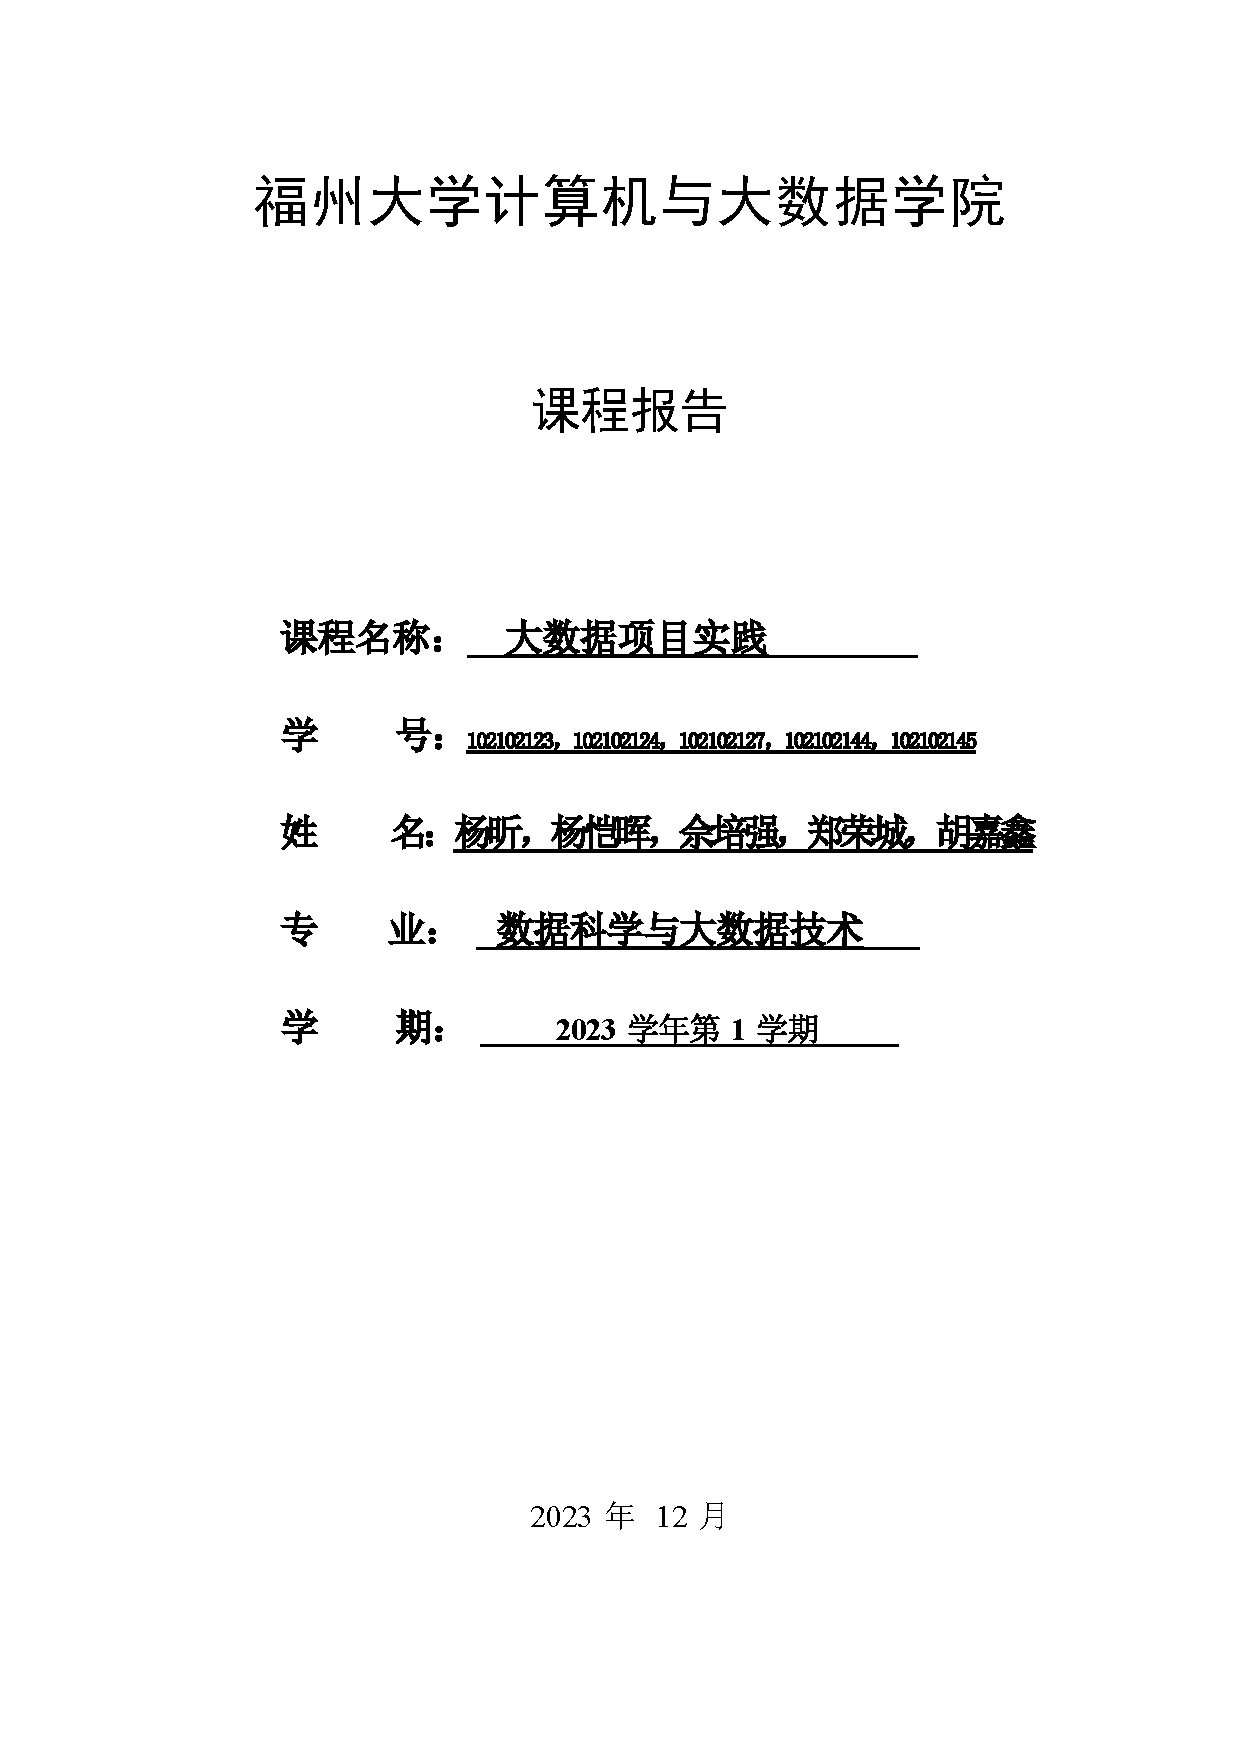
\includepdf[pages=1-1]{./resources/cover.pdf}

% XXXXXXX(题目)
\maketitle

% 摘要
% 摘 要:
% 描述选题背景、课题任务的总结、特色或意义的阐述。
% (500 字左右,单独 1 页)
% 建议: 课题任务包括 大数据计算方法(算法)+原型系统(模块)开发
\begin{abstract}
在蚂蚁集团的大数据应用场景中,尤其是金融风控、实时数仓等场景下,存在大量Join运算,如何提高Join
的时效性和性能成为重要挑战,为此引入了图模型。图模型是一种以点边结构描述实体关系的数据模型,在图模型里面,点代表实体,
边代表关系,数据存储层面点边存放在一起。因此,图模型天然定义了数据的关系同时存储层面物化了点边关系。基于图模型,蚂蚁集团实现了新一代实时计算 引擎GeaFlow,很好的解决了复杂关系运算实时化的问题。目前GeaFlow已广泛应用于数仓加速、金融风控、知识图谱以及社交网络等场景。

图模式匹配是一种在图结构中寻找与给定模式相同或相似子图的技术,是图计算领域中一类非常经典的算法问题,在金融风控、社交推荐、计算机视觉、生物信息学等领域有着广泛的应用场景。
随着图数据规模的增大,图模式匹配的计算和存储成本急剧上升,基于分布式图计算引擎提供的迭代计算框架,是实现大规模图数据上图模式匹配算法的一种常用手段。

本文基于蚂蚁开源的分布式实时图计算引擎TuGraph Analytics提供的⾼阶API编程接口,
在LDBC FinBench测试数据集上,完成指定的图模式匹配算法的实现,并尽可能提升算法的整体性能(包含构图、匹配、输出全部过程)。
\end{abstract}

\newpage

%目录(插入对应目录,并及时更新)
\tableofcontents

% 1 引言
% (阐述课题研发的详细背景、应用场景、问题、可能的解决的思路与技术概述等….)
\section{引言}

\subsection{历史背景}
早期的大数据分析主要以离线处理为主,以Hadoop为代表的技术栈很好的解决了大规模数据的分析问题。
然而数据处理的时效性不足, 很难满足高实时需求的场景。
以Storm为代表的流式计算引擎的出现则很好的解决了数据实时处理的问题,提高了数据处理的时效性。
然而,Storm 本身不提供状态管理的能力, 对于聚合等有状态的计算显得无能为力。
Flink 的出现很好的弥补了这一短板,通过引入状态管理以及 Checkpoint 机制,实现了高效的有状态流计算能力。

随着数据实时处理场景的丰富,尤其是在实时数仓场景下,实时关系运算(即 Stream Join) 越来越多的成为数据实时化的难点。
Flink 虽然具备优秀的状态管理能和出色的性能,然而在处理 Join 运算,尤其是3度以上Join时, 性能瓶颈越来越明显。
由于需要在Join两端存放各个输入的数据状态,当Join变多时,状态的数据量急剧扩大,性能也变的难以接受。
产生这个问题的本质原因是Flink等流计算系统以表作为数据模型,而表模型本身是一个二维结构,不包含关系的定义和关系的存储, 在处理关系运算时只能通过Join运算方式实现,成本很高。

\subsection{应用场景}
在蚂蚁集团的大数据应用场景中,尤其是金融风控、实时数仓等场景下,存在大量Join运算,如何提高Join
的时效性和性能成为重要挑战,为此引入了图模型。图模型是一种以点边结构描述实体关系的数据模型,在图模型里面,点代表实体,
边代表关系,数据存储层面点边存放在一起。因此,图模型天然定义了数据的关系同时存储层面物化了点边关系。
基于图模型,蚂蚁集团实现了新一代实时计算 引擎GeaFlow,很好的解决了复杂关系运算实时化的问题。目前GeaFlow已广泛应用于数仓加速、金融风控、知识图谱以及社交网络等场景。

图模式匹配是一种在图结构中寻找与给定模式相同或相似子图的技术,是图计算领域中一类非常经典的算法问题,在金融风控、社交推荐、计算机视觉、生物信息学等领域有着广泛的应用场景。
随着图数据规模的增大,图模式匹配的计算和存储成本急剧上升,基于分布式图计算引擎提供的迭代计算框架,是实现大规模图数据上图模式匹配算法的一种常用手段。

\subsection{问题概述}
本文基于蚂蚁开源的分布式实时图计算引擎TuGraph Analytics提供的⾼阶API编程接口,
在LDBC FinBench测试数据集上,完成指定的图模式匹配算法的实现,并尽可能提升算法的整体性能(包含构图、匹配、输出全部过程)。

\subsection{解决思路概述}
\begin{enumerate}
  \item Input: 图构建;
  \item Processing: 图匹配;
  \item Output: 处理中间结果并得到输出.
\end{enumerate}

% 2 国内外现状 或 相关研发情况
% (该部分的书写内容及标题等根据情况确定,或者删除该部分内容)
\section{相关研发情况}
\subsection{Geaflow整体架构}
GeaFlow 整体架构如下所示:
\begin{figure}[H]
  \begin{center}
    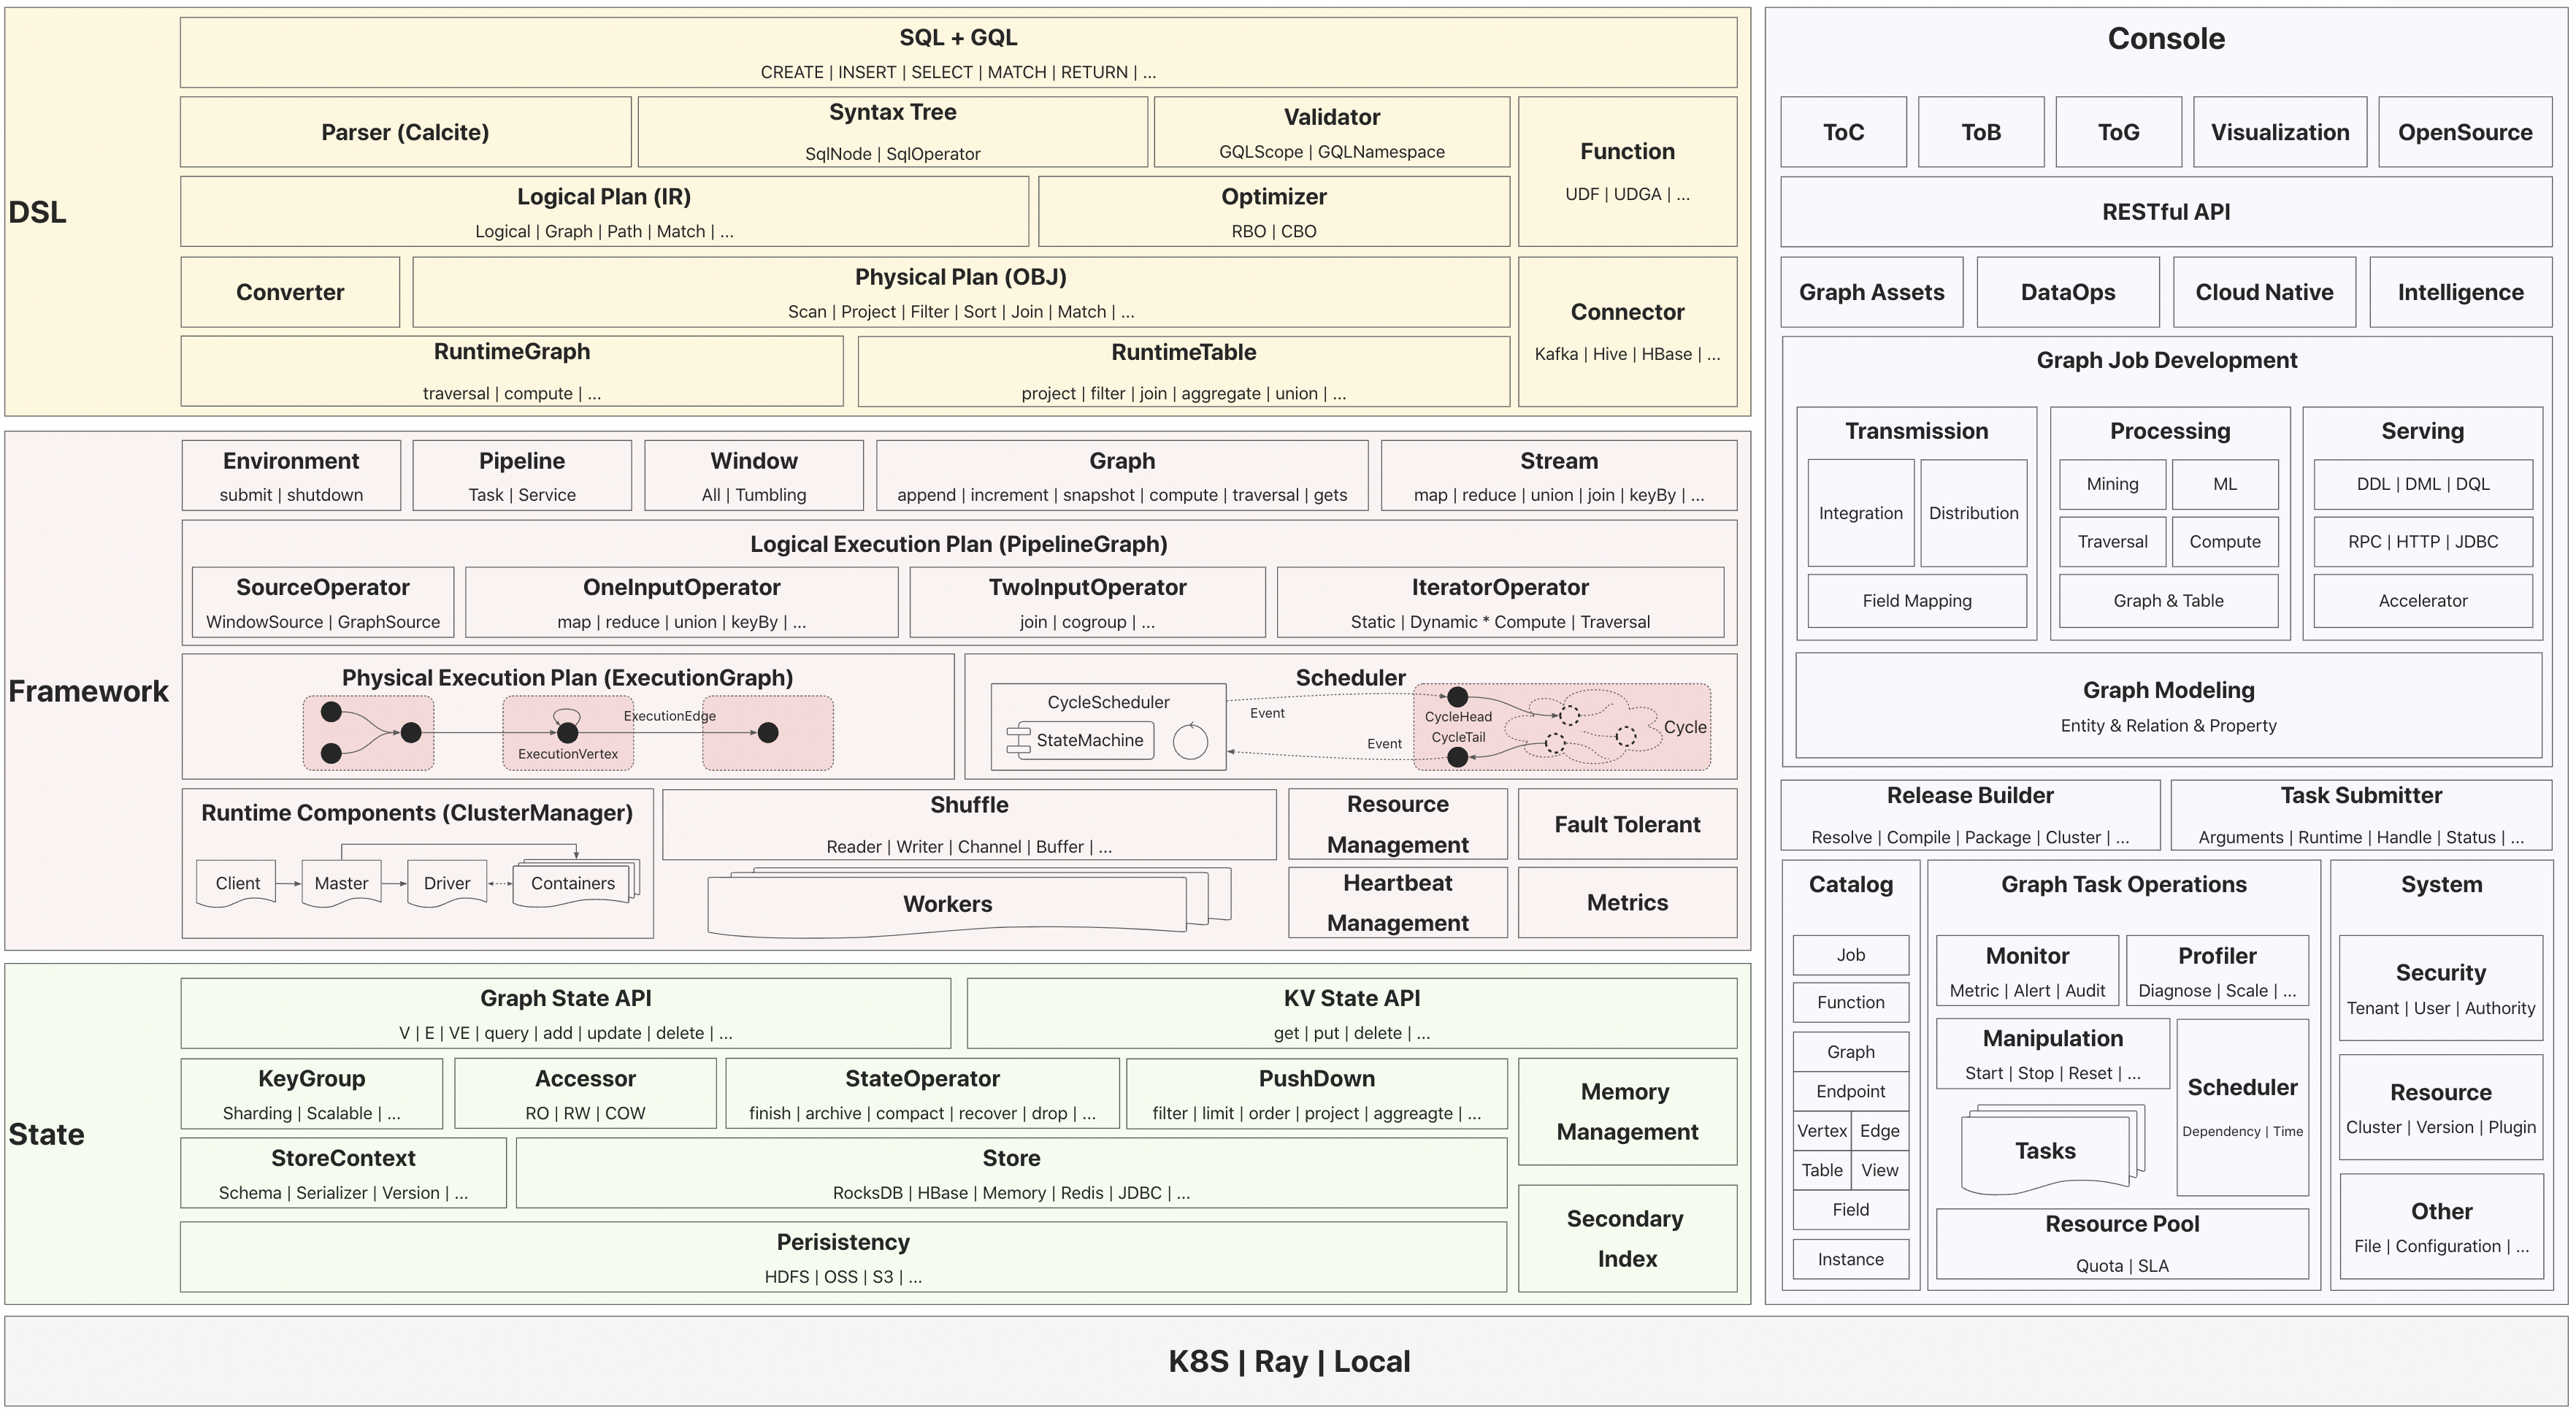
\includegraphics[width=0.90\textwidth]{./figures/geaflow_arch_new.png}
  \end{center}
  \caption{Geaflow 技术架构}
\end{figure}

\begin{itemize}
  \item DSL层:即语言层。GeaFlow设计了SQL+GQL的融合分析语言,支持对表模型和图模型统一处理。
  \item Framework层:即框架层。GeaFlow设计了面向Graph和Stream的两套API支持流、批、图融合计算,并实现了基于Cycle的统一分布式调度模型。
  \item State层:即存储层。GeaFlow设计了面向Graph和KV的两套API支持表数据和图数据的混合存储,整体采用了Sharing Nothing的设计,并支持将数据持久化到远程存储。
  \item Console平台:GeaFlow提供了一站式图研发平台,实现了图数据的建模、加工、分析能力,并提供了图作业的运维管控支持。
  \item 执行环境:GeaFlow可以运行在多种异构执行环境,如K8S、Ray以及本地模式。
\end{itemize}

\subsection{GeaFlow API 介绍}
GeaFlow API是对高阶用户提供的开发接口,其支持Graph API和Stream API两种类型:
\begin{figure}[H]
  \begin{center}
    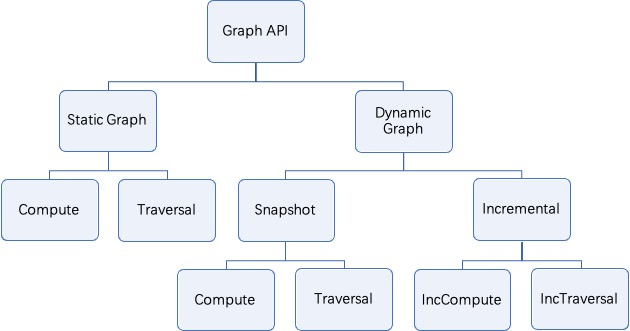
\includegraphics[width=0.65\textwidth]{./figures/api_arch.jpeg}
  \end{center}
  \caption{Geaflow API 介绍}
\end{figure}
\begin{itemize}
  \item Graph API:Graph是GeaFlow框架的一等公民,当前GeaFlow框架提供了一套基于GraphView的图计算编程接口,
    包含图构建、图计算及遍历。在GeaFlow中支持Static Graph和Dynamic Graph两种类型。
  \item Static Graph API:静态图计算API,基于该类API可以进行全量的图计算或图遍历。
  \item Dynamic Graph API:动态图计算API,GeaFlow中GraphView是动态图的数据抽象,基于GraphView之上,可以进行动态图计算或图遍历。
    同时支持对Graphview生成Snapshot快照,基于Snapshot可以提供和Static Graph API一样的接口能力。
  \item Stream API:GeaFlow提供了一套通用计算的编程接口,包括source构建、流批计算及sink输出。
    在GeaFlow中支持Batch和Stream两种类型。
  \item Batch API:批计算API,基于该类API可以进行批量计算。
  \item Stream API:流计算API,GeaFlow中StreamView是动态流的数据抽象,基于StreamView之上,可以进行流计算。
\end{itemize}

通过两种类型API的介绍可以看到,GeaFlow内部通过View统一了图视图和流视图语义。
同时为了统一支持动态和静态计算两套API,GeaFlow内部抽象了Window的概念,
即从Source API开始就必须带有Window,用以基于Window的方式切分数据窗口。

\begin{itemize}
  \item 对流或动态图API来说,Window可以按照 size 来切分,每个窗口读取一定size的数据,从而实现流式增量的计算。
  \item 对批或静态图API来说,Window将采用AllWindow模式,一个窗口将读取全量数据,从而实现全量的计算。
\end{itemize}

本文主要使用 Geaflow API 的 Graph API, Graph API是GeaFlow中的一等公民,其提供了一套基于GraphView的图计算编程接口,包含图构建、图计算及遍历。
关于 Stream API 的详细内容可参见 GeaFlow 官网\cite{ref1}.

\subsection{Graph API}
静态图:
\begin{table}[H]
  \caption{静态图}
  \begin{center}
    \begin{tabularx}{\textwidth}{Xl}
      \toprule
      \textbf{API} & \textbf{说明} \\
      \midrule
      \texttt{PGraphCompute compute(VertexCentricCompute vertexCentricCompute)} & 在Graph上进行静态图VC计算 \\
      \texttt{PGraphWindow compute(ScatterGatherCompute sgAlgorithm, int parallelism)} & 在Graph上进行静态图SG计算 \\
      \texttt{PWindowStream getEdges()} & 返回edge集合 \\
      \texttt{PWindowStream getVertices()} & 返回vertex集合 \\
      \bottomrule
    \end{tabularx}
  \end{center}
\end{table}

\subsubsection{Compute API 介绍}
GeaFlow对外提供了实现图计算算法的接口,通过实现相应接口可进行静态图计算或动态图计算,用户可在compute算法中定义具体的计算逻辑及迭代最大次数。

本文主要使用 Geaflow 的静态图接口.

静态图接口:
\begin{table}[H]
  \caption{静态图接口}
  \begin{center}
    \begin{tabularx}{\textwidth}{XlX}
      \toprule
      \textbf{API} & \textbf{接口说明} & \textbf{入参说明} \\
      \midrule
      \texttt{void init(\newline VertexCentricComputeFuncContext vertexCentricFuncContext)}
                   & 迭代计算初始化接口
                   & vertexCentricFuncContext: 静态图计算的上下文, K 表示 vertex
                   id 的类型,VV 表示 vertex value 类型,EV 表示 edge
                   value 类型,M 表示发送消息的类型。 \\
      \texttt{void compute(K vertexId, Iterator messageIterator)}
                   & 迭代计算接口
                   & vertexId: 当前计算点 id, 其中 K 表示 vertexId 的类型。
                   messageIterator: 迭代过程中所有发送给当前点的消息,
                   M 表示迭代计算过程中定义的发送消息类型。 \\
      \texttt{void finish()}
                   & 迭代计算完成接口
                   & - \\
      \bottomrule
    \end{tabularx}
  \end{center}
\end{table}

详细接口:
\begin{center}
\begin{minted}[xleftmargin=5mm]{java}
public interface VertexCentricComputeFunction<K, VV, EV, M>
  extends VertexCentricFunction<K, VV, EV, M> {
  void init(VertexCentricComputeFuncContext<K, VV, EV, M> vertexCentricFuncContext);
  void compute(K vertex, Iterator<M> messageIterator);
  void finish();

  interface VertexCentricComputeFuncContext<K, VV, EV, M>
    extends VertexCentricFuncContext<K, VV, EV, M> {
      /* 设置vertex value */
      void setNewVertexValue(VV value);
  }
}
\end{minted}
\end{center}

\section{数学模型}

\subsection{图的抽象}
% TODO:

\subsection{名称解释}
\begin{itemize}
  \item 图: 图用于展示不同变量之间的关系,通常包括节点(点)和边(线)两部分。
    节点代表一个个体或对象,边则代表它们之间的关系。图可以用来解释复杂的关系网络和信息流动,
    如社交网络、交通网络、物流网络等。常见的图形类型包括有向图、无向图、树形图、地图等。
  \item Graph Processing:  Graph Processing是一种计算模型,用于处理图形数据结构的计算问题。
    图计算模型可以用于解决许多现实世界的问题,例如社交网络分析、网络流量分析、医疗诊断等,
    典型的系统有 Apache Giraph, Spark GraphX。
  \item DSL:  DSL是领域特定语言(Domain Specific Language)的缩写。
    它是一种针对特定领域或问题的编程语言,与通用编程语言不同,DSL主要关注于解决特定领域的问题,并针对该领域的特定需求进行优化。
    DSL可以使得编程更加简单、高效,同时也能够提高代码的可读性和可维护性。下面的Gremlin、ISO GQL就是DSL中的一种。
  \item HLA: HLA 是 High level language 的缩写,与DSL不同,它使用通用语言进行编程,Geaflow目前只支持Java程序编写。
    它主要通过计算引擎SDK进行程序编写,执行方式是将程序整体打包交给引擎执行,对比DSL,它的执行方式更加灵活,但相对应的编程也会更加复杂。
  \item Gremlin: Gremlin是一种图形遍历语言,用于在图形数据库中进行数据查询和操作。
    它是一种声明式的、基于图的编程语言,可以用于访问各种类型的图形数据库,如Apache TinkerPop、Neo4j等。
    它提供了一组灵活的API,可以帮助开发者在图形数据库中执行各种操作,如遍历、过滤、排序、连接、修改等。
  \item ISO GQL: GQL是面向属性图的标准查询语言,全称是“图形查询语言”,其为ISO/IEC国际标准数据库语言。
    GeaFlow不仅支持了Gremlin查询语言,而且还支持了GQL。
  \item Window: 参考VLDB 2015 Google Dataflow Model,窗口的概念在 Geaflow 中是其数据处理逻辑中的关键要素,用于统一有界和无界的数据处理。
    数据流统一被看成一个个窗口数据的集合,系统处理批次的粒度也就是窗口的粒度。
  \item Cycle: GeaFlow Scheduler调度模型中的核心数据结构,一个cycle描述为可循环执行的基本单元,包含输入,中间计算和数据交换,输出的描述。
    由执行计划中的vertex group生成,支持嵌套。
  \item Event: Runtime层调度和计算交互的核心数据结构,Scheduler将一系列Event集合构建成一个State Machine,将其分发到Worker上进行计算执行。
    其中有些Event是可执行的,即自身具备计算语义,整个调度和计算过程为异步执行。
  \item Graph Traversal: Graph Traversal 是指遍历图数据结构中所有节点或者部分节点的过程,在特定的顺序下访问所有节点,
    主要是深度优先搜索(DFS)和 广度优先搜索(BFS)。用于解决许多问题,包括查找两个节点之间的最短路径、检测图中的循环等。
  \item Graph State:  GraphState 是用来存放Geaflow的图数据或者图迭代计算过程的中间结果,提供Exactly Once语义,并提供作业级复用的能力。
    GraphState 分为 Static 和 Dynamic 两种,Static 的 GraphState 将整个图看做是一个完整的,
    所有操作都在一张全图上进行;Dynamic 的 GraphState 认为图动态变化的,由一个个时间切片构成,所有切片构成一个完整的图,
    所有的操作都是在切片上进行。
  \item Key State:  KeyState 用于存放计算过程中的中间结果,通常用于流式处理,例如执行aggregation时在KeyState中记录中间聚合结果。
    类似GraphState,Geaflow 会将 KeyState 定期持久化,因此KeyState也提供Exactly Once语义。
    KeyState根据数据结果不同可以分为KeyValueState、KeyListState、KeyMapState等。
\end{itemize}

\section{问题描述}
\subsection{概述}
基于蚂蚁开源的分布式实时图计算引擎TuGraph Analytics提供的⾼阶API编程接口,在LDBC FinBench测试数据集上,完成赛题指定的图模式匹配算法的实现,并尽可能提升算法的整体性能(包含构图、匹配、输出全部过程)。

\subsection{数据简介}
基于TuGraph Analytics的高阶API进行构图操作,将``FinBench数据集''转换为以下图数据格式。

\subsection{数据格式}
具体数据格式信息可参考``LDBC FinBench文档''\cite{ref3} Data Definition 章节.

\begin{figure}[H]
  \begin{center}
    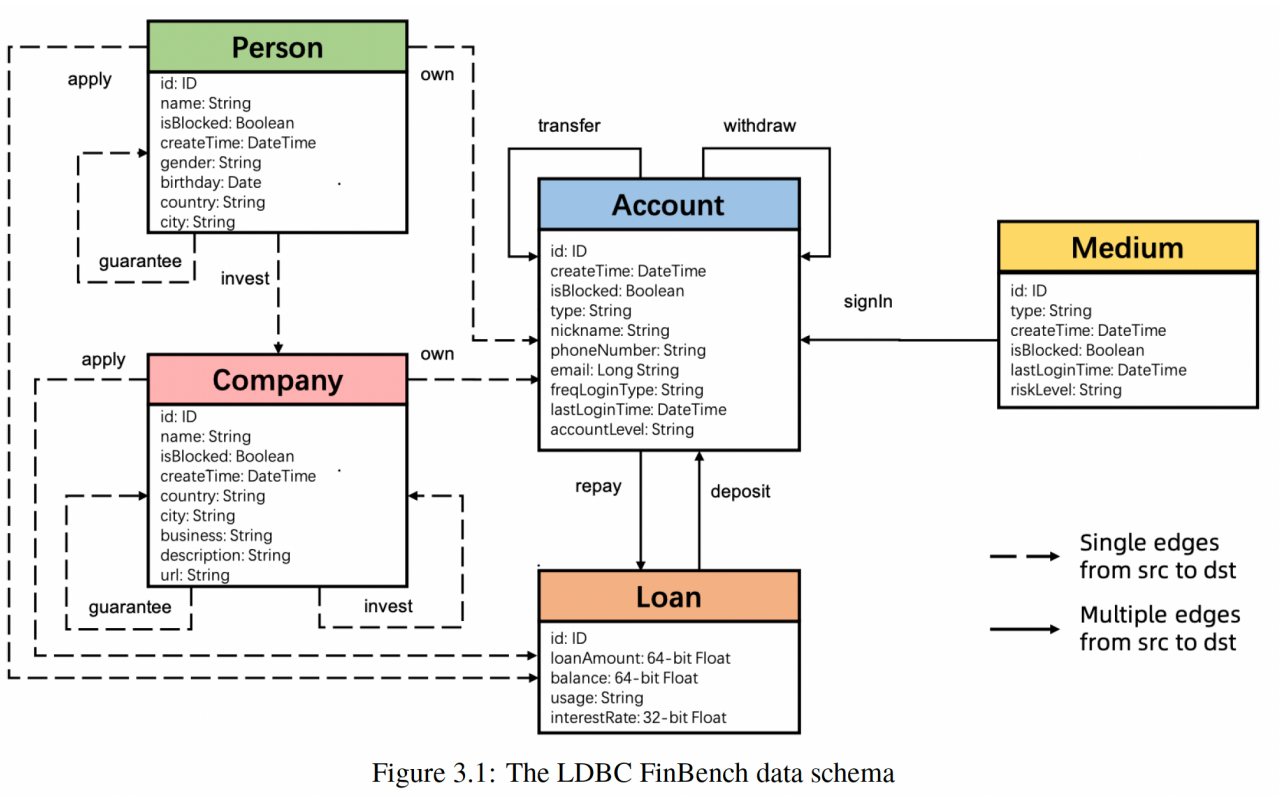
\includegraphics[width=0.95\textwidth]{./figures/蚂蚁2-1-728694.png}
  \end{center}
  \caption{The LDBC FinBench data schema}
\end{figure}

\subsection{数据文件}
\begin{itemize}
  \item 点数据文件:
    \begin{enumerate}
      \item Account.csv
      \item Loan.csv
      \item Person.csv
    \end{enumerate}
  \item 边数据文件:
    \begin{enumerate}
      \item AccountTransferAccount.csv
      \item LoanDepositAccount.csv
      \item PersonApplyLoan.csv
      \item PersonGuaranteePerson.csv
      \item PersonOwnAccount.csv
    \end{enumerate}
\end{itemize}

\subsection{交易闭环搜索问题}
\begin{figure}[H]
  \begin{center}
    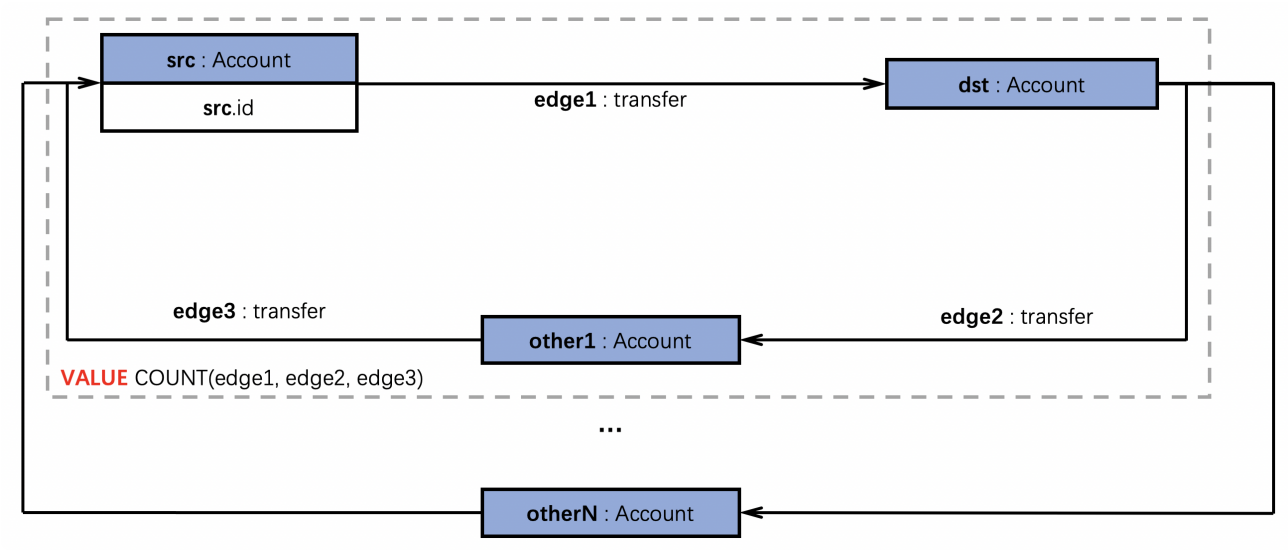
\includegraphics[width=0.95\textwidth]{./figures/蚂蚁改5-264319.png}
  \end{center}
  \caption{交易闭环搜索}
\end{figure}

\begin{itemize}
  \item 目标: 匹配满足以下条件的所有账户src:
    \begin{enumerate}
      \item src 向账户 dst 发起过转账(edge1:transfer)。
      \item dst 向另一个账户 other 发起过转账(edge2:transfer)。
      \item other 向 src 发起过转账(edge3:transfer)。
    \end{enumerate}
  \item 输出
    \begin{enumerate}
      \item id:满足目标条件的 src.id。
      \item value:交易闭环(序列<edge1, edge2, edge3>)中的数量。
    \end{enumerate}
\end{itemize}

\subsection{资金快进快出问题}
\begin{figure}[H]
  \begin{center}
    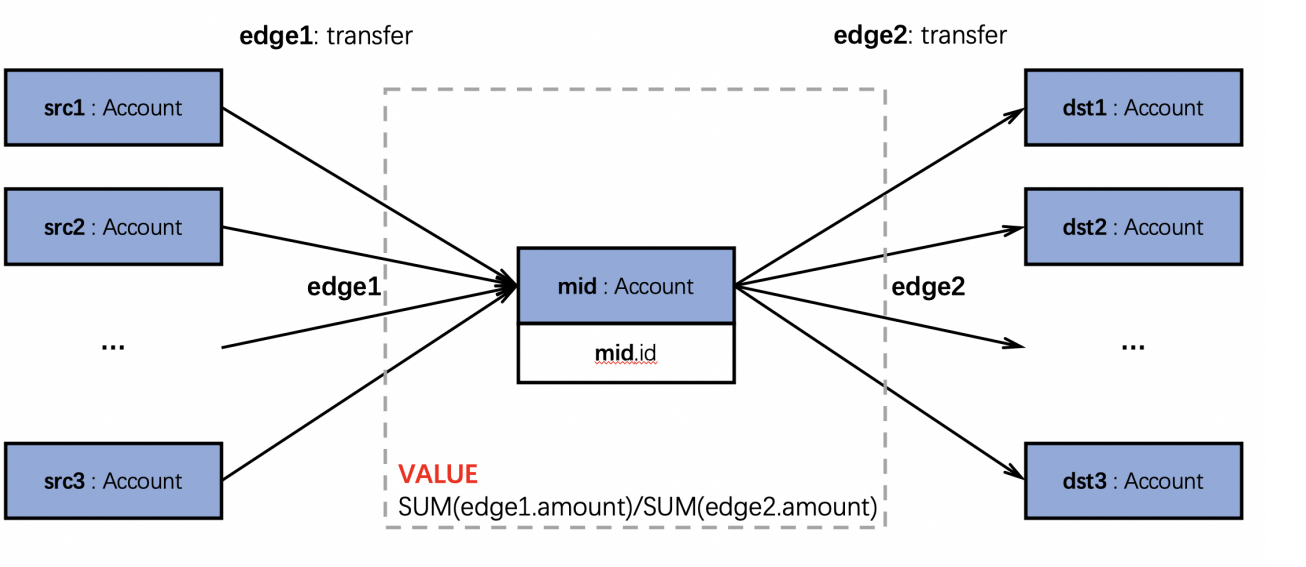
\includegraphics[width=0.95\textwidth]{./figures/蚂蚁改6-546936.png}
  \end{center}
  \caption{资金快进快出}
\end{figure}

\begin{itemize}
  \item 目标: 匹配满足以下条件的所有账户mid:
    \begin{enumerate}
      \item 找到所有向mid发起的转账边(edge1:transfer),至少一条。
      \item 找到所有mid发起的转账边(edge2:transfer),至少一条。
    \end{enumerate}
  \item 输出
    \begin{enumerate}
      \item id:满足目标条件的 mid.id。
      \item value:交易流入流出比,SUM(edge1.amount) / SUM(edge2.amount),小数点后保留2位有效数字。
    \end{enumerate}
\end{itemize}

\subsection{结果格式}
\begin{itemize}
  \item 每个 Case 的结果写到单独的 CSV 文件,文件名为:``result'' + \$\{Case编号\} +
    ``.csv'',如 result1.csv。
  \item 文件内容格式为:
    \begin{enumerate}
      \item 分隔符统一使用:|;
      \item 首行必须是:id|value;
      \item 其中 id 要保证自增顺序(按照数字大小进行排序).
    \end{enumerate}
\end{itemize}

\subsection{测试环境}
\begin{itemize}
  \item CPU: 16vCPU;
  \item 内存: 64 GB;
  \item 硬盘: 满足需求即可.
\end{itemize}

\section{问题求解}
\subsection{开发环境搭建}
\begin{itemize}
  \item 安装 JDK8(GeaFlow 目前只支持 JDK8), 包括配置相应的环境变量.
  \item 安装 Maven, 包括配置相应的环境变量.
  \item 安装任意可以编写代码的文本编辑器.
  \item 下载数据集到本地磁盘.
\end{itemize}

添加 Maven 坐标(完整配置可见项目源码的 pom.xml 文件):
\begin{center}
\begin{minted}[xleftmargin=5mm]{xml}
<dependency>
    <groupId>com.antgroup.tugraph</groupId>
    <artifactId>geaflow-api</artifactId>
    <version>0.3</version>
</dependency>

<dependency>
    <groupId>com.antgroup.tugraph</groupId>
    <artifactId>geaflow-pdata</artifactId>
    <version>0.3</version>
</dependency>

<dependency>
    <groupId>com.antgroup.tugraph</groupId>
    <artifactId>geaflow-cluster</artifactId>
    <version>0.3</version>
</dependency>

<dependency>
    <groupId>com.antgroup.tugraph</groupId>
    <artifactId>geaflow-on-local</artifactId>
    <version>0.3</version>
</dependency>

<dependency>
    <groupId>com.antgroup.tugraph</groupId>
    <artifactId>geaflow-pipeline</artifactId>
    <version>0.3</version>
</dependency>
\end{minted}
\end{center}

打包:
\begin{center}
\begin{minted}[xleftmargin=5mm]{bash}
mvn clean package -DskipTests
\end{minted}
\end{center}

运行:
\begin{center}
\begin{minted}[xleftmargin=5mm]{bash}
$JAVA_HOME/bin/java -jar target/*.jar 数据集路径 结果文件路径
\end{minted}
\end{center}

\subsection{通用的类和函数}
由于问题是基于 GeaFlow API 进行图构建和计算的, 对于不同的问题,
仅仅是点和边的数据发生改变, 构图的 API 是相似的, 为此我们抽象出
求解各个问题的通用类和函数.

\subsubsection{图输入}
具体输入数据的格式可见问题描述一节, 此处不再赘述.
相关依赖的导入请见相关源码文件, 此处为避免篇幅过长, 故省略之.

\begin{center}
\begin{minted}[xleftmargin=5mm]{java}
package org.graphpatmatch.yyds.utils;

public class FileSource<OUT>
  extends RichFunction implements SourceFunction<OUT> {
  // 文件名
  protected String filePath;
  // 输入文件的路径
  public static final String INPUT_DIR = "input.dir";
  // 读入的数据
  protected List<OUT> records;
  protected Integer readPos = null;
  // 读入数据的解析器
  protected FileLineParser<OUT> parser;
  protected transient RuntimeContext runtimeContext;

  public FileSource(String filePath, FileLineParser<OUT> parser) {
    this.filePath = filePath;
    this.parser = parser;
  }

  @Override
  public void open(RuntimeContext runtimeContext) {
    this.runtimeContext = runtimeContext;
    filePath = String.format("%s/%s",
        runtimeContext.getConfiguration().getString("input.dir"), filePath);
  }

  @Override
  public void init(int parallel, int index) {
    this.records = readFileLines(filePath);
    if (parallel != 1) {
      List<OUT> allRecords = records;
      records = new ArrayList<>();
      for (int i = 0; i < allRecords.size(); i++) {
        if (i % parallel == index) {
          records.add(allRecords.get(i));
        }
      }
    }
  }

  @Override
  public boolean fetch(IWindow<OUT> window, SourceContext<OUT> ctx)
    throws Exception {
    if (readPos == null) {
      readPos = 0;
    }
    while (readPos < records.size()) {
      OUT out = records.get(readPos);
      long windowId = window.assignWindow(out);
      if (window.windowId() == windowId) {
        ctx.collect(out);
        readPos++;
      } else {
        break;
      }
    }
    boolean result = false;
    if (readPos < records.size()) {
      result = true;
    }
    return result;
  }

  // 以行为单位读入数据
  private List<OUT> readFileLines(String filePath) {
    try {
      List<String> lines = Files.readLines(new File(filePath),
          Charset.defaultCharset());
      List<OUT> result = new ArrayList<>();

      // 过滤掉首行(header)
      lines.remove(0);

      for (String line : lines) {
        if (StringUtils.isBlank(line)) {
          continue;
        }
        Collection<OUT> collection = parser.parse(line);
        result.addAll(collection);
      }
      return result;
    } catch (IOException e) {
      throw new RuntimeException("error in read resource file: " + filePath, e);
    }
  }

  public interface FileLineParser<OUT> extends Serializable {
    Collection<OUT> parse(String line);
  }
}
\end{minted}
\end{center}

\subsubsection{图输出}
\begin{center}
\begin{minted}[xleftmargin=5mm]{java}
package org.graphpatmatch.yyds.utils;

public class FileSink<OUT>
  extends RichFunction implements SinkFunction<OUT> {
  // 输出文件路径
  public static final String OUTPUT_DIR = "output.dir";
  // 输出文件名
  public static final String OUTPUT_FILE = "output.file";
  public static final String FILE_OUTPUT_APPEND_ENABLE = "file.append.enable";
  private Boolean first = false;
  private File file;

  public FileSink() {
  }

  @Override
  public void open(RuntimeContext runtimeContext) {
    String filePath = String.format("%s/%s",
        runtimeContext.getConfiguration().getString(OUTPUT_DIR),
        runtimeContext.getConfiguration().getString(OUTPUT_FILE));

    boolean append = runtimeContext.getConfiguration()
      .getBoolean(new ConfigKey(FILE_OUTPUT_APPEND_ENABLE, true));
    file = new File(filePath);

    // 若指定的文件不存在, 则创建之
    try {
      if (!append && file.exists()) {
        try {
          FileUtils.forceDelete(file);
        } catch (Exception e) {
          // ignore
        }
      }

      if (!file.exists()) {
        if (!file.getParentFile().exists()) {
          file.getParentFile().mkdirs();
        }
        file.createNewFile();
      }
    } catch (IOException e) {
      throw new GeaflowRuntimeException(e);
    }
  }

  @Override
  public void write(OUT out) throws Exception {
    try {
      // 写入首行(header)
      if (!first) {
        FileUtils.write(file, "id|value\n", Charset.defaultCharset(), true);
        first = true;
      }
      // 逐行写入
      FileUtils.write(file, out + "\n", Charset.defaultCharset(), true);
    } catch (IOException e) {
      throw new RuntimeException(e);
    }
  }
}
\end{minted}
\end{center}

\subsubsection{输出排序}
结果文件要求输出按照 id 的数值大小进行升序排序, 我们在此处说明排序的逻辑.

\begin{center}
\begin{minted}[xleftmargin=5mm]{java}
package org.graphpatmatch.yyds.utils;

public class FileSort {
  public static void sort(String TMP_FILE, String RESULT_FILE) {
    try {
      // 中间文件
      File fin = new File(TMP_FILE);
      // 结果文件
      File fout = new File(RESULT_FILE);

      FileInputStream fis = new FileInputStream(fin);
      FileOutputStream fos = new FileOutputStream(fout);

      BufferedReader in = new BufferedReader(new InputStreamReader(fis));
      BufferedWriter out = new BufferedWriter(new OutputStreamWriter(fos));

      String aLine;
      // 有序映射, <id, value>: <BigInteger, String>
      SortedMap<BigInteger, String> sortedMap = new TreeMap<BigInteger, String>();

      in.readLine(); // Skip the first line(header)
      while ((aLine = in.readLine()) != null) {
        if (aLine.trim().length() > 0) { // 非空行
          // split() 根据正则表达式进行分割, | 是正则表达式的元字符, 故需转义
          sortedMap.put(new BigInteger(aLine.split("\\|")[0]), aLine);
        }
      }

      out.write("id|value\n"); // Write header
      Set<Entry<BigInteger, String>> entries = sortedMap.entrySet();
      for (Entry<BigInteger, String> entry : entries) {
        out.write(entry.getValue() + "\n");
      }

      in.close();
      out.close();
      // 删除临时文件
      FileUtils.forceDelete(new File(TMP_FILE));
    } catch (IOException e) {
    }
  }
}
\end{minted}
\end{center}

程序运行时环境的初始化和参数配置请见源码, 以下仅描述
构图过程和核心算法.

\subsection{交易闭环搜索问题}
具体问题描述可见 \ref{pro1} 交易闭环搜索问题 一节.

此问题涉及的数据文件有:
\begin{itemize}
  \item Account.csv(点)
  \item AccountTransferAccount.csv(边)
\end{itemize}

\subsubsection{输入}
\begin{center}
\begin{minted}[xleftmargin=5mm]{java}
// 构建点
PWindowSource<IVertex<String, Integer>> vertices = pipelineTaskCxt
  .buildSource(
    new FileSource<IVertex<String, Integer>>(
      "Account.csv",
      line -> {
        String[] fields = line.split("\\|");
        // <vertexKey, vertexValue>: <String, Integer>
        // 此处以 Account 的 Id 作为点的 Id,
        // 点的值为以此点为源点的三角形的个数
        IVertex<String, Integer> vertex = new ValueVertex<String, Integer>(
        fields[0], 0);
        return Collections.singletonList(vertex);
    }),
    AllWindow.getInstance())
  .withParallelism(sourceParallelism);

// 构建边
PWindowSource<IEdge<String, String>> edges = pipelineTaskCxt
  .buildSource(
    new FileSource<IEdge<String, String>>(
      "AccountTransferAccount.csv",
      line -> {
        String[] fields = line.split("\\|");
        // <vertexKey, edgeValue>: <String, String>
        // 此处以 Account 的 Id 作为点的 Id
        IEdge<String, String> edge = new ValueEdge<String, String>(
          fields[0], fields[1], ""); // (srcId, targetId, edgeValue)
        return Collections.singletonList(edge);
    }),
    AllWindow.getInstance())
  .withParallelism(sourceParallelism);

// 构造图视图(用于将构造出的点和边关联起来)
GraphViewDesc graphViewDesc = GraphViewBuilder
  .createGraphView(GraphViewBuilder.DEFAULT_GRAPH)
  .withShardNum(iterationParallelism)
  .withBackend(BackendType.Memory)
  .build();
\end{minted}
\end{center}

\subsubsection{核心算法}
此问题可看作是寻找图中三角形 $ K^{3} $ 的个数.

对图中的某个点 $ A $, $ A $ 向每个相邻点发送消息 $ M=(1, A) $, 此后消息
$ M $ 每传递一次, $ M $ 的第一个元素的值就增加 $ 1 $, 若 $ A $ 在某个三角形中,
则 $ M $ 最终会被传回给 $ A $, 此时 $ M = (3, A) $, 点 $ A $
发现这是自己发出的消息, 于是更新状态(以 $ A $ 为源点的三角形个数);
若 $ M $ 的第一个元素的值为 $ 3 $ 且消息到达的点的 Id 与 $ M $ 的第二个元素不等,
则丢弃该消息, 不再继续传递.

\begin{figure}[H]
  \begin{center}
    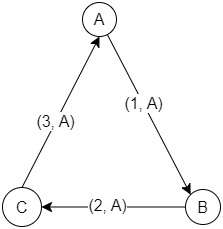
\includegraphics[width=0.15\textwidth]{./figures/pro1.jpg}
  \end{center}
  \caption{交易闭环搜索消息传递}
\end{figure}

\begin{center}
\begin{minted}[xleftmargin=5mm]{java}
public void compute(
  String vertexId, Iterator<String> messageIterator) {
  IVertex<String, Integer> vertex = this.context.vertex().get();

  // 首轮迭代向所有相邻节点发送消息
  if (this.context.getIterationId() == 1L) {
    this.context.sendMessageToNeighbors("1," + vertexId);
  }

  while (messageIterator.hasNext()) {
    String[] msg = messageIterator.next().split(",");
    int t = Integer.parseInt(msg[0]);
    String msgId = msg[1];

    if (t < 3) {
      t += 1;
      if (t == 3) {
        List<IEdge<String, String>> edges = this.context
          .edges().getOutEdges();
        for (IEdge<String, String> edge : edges) {
          if (msgId.equals(edge.getTargetId())) {
            // 仅向可以形成闭环的点发送消息,
            // 避免非必要的内存浪费和减少计算的时间开销
            this.context.sendMessage(msgId, "3," + msgId);
          }
        }
      } else {
        this.context.sendMessageToNeighbors(
          Integer.toString(t) + "," + msgId);
      }
    } else if (t == 3) { // 找到一个闭环, 更新结果
      this.context.setNewVertexValue(vertex.getValue() + 1);
    }
  }
}
\end{minted}
\end{center}

\subsubsection{输出}
\begin{center}
\begin{minted}[xleftmargin=5mm]{java}
PWindowStream<IVertex<String, Integer>> result = pipelineTaskCxt
  .buildWindowStreamGraph(vertices, edges, graphViewDesc)
  .compute(new Case2Algorithms(4)) // 迭代 4 轮
  .compute(iterationParallelism)
  .getVertices();

SinkFunction<String> sink = ExampleSinkFunctionFactory
  .getSinkFunction(conf);
result
  .filter(v -> v.getValue() >= 1) // 过滤出符合要求的点
  .map(v -> String.format("%s|%s", v.getId(), v.getValue()))
  .withParallelism(mapParallelism)
  .sink(sink) // 写入文件
  .withParallelism(sinkParallelism);
\end{minted}
\end{center}

\subsection{资金快进快出问题}
具体问题描述可见 \ref{pro2} 资金快进快出问题一节.

此问题涉及的数据文件有:
\begin{itemize}
  \item Account.csv(点)
  \item AccountTransferAccount.csv(边)
\end{itemize}

\subsubsection{输入}
\begin{center}
\begin{minted}[xleftmargin=5mm]{java}
// 构建点
PWindowSource<IVertex<String, String>> vertices = pipelineTaskCxt
  .buildSource(
    new FileSource<IVertex<String, String>>(
      "Account.csv",
      line -> {
        String[] fields = line.split("\\|");
        // <vertexKey, vertexValue>: <String, String>
        // 此处以 Account 的 Id 作为点的 Id,
        IVertex<String, String> vertex = new ValueVertex<String, String>(
          fields[0], "");
        return Collections.singletonList(vertex);
    }),
    AllWindow.getInstance())
  .withParallelism(sourceParallelism);

// 构建边
PWindowSource<IEdge<String, Double>> edges = pipelineTaskCxt
  .buildSource(
    new FileSource<IEdge<String, Double>>(
      "AccountTransferAccount.csv",
      line -> {
        String[] fields = line.split("\\|");
        // <vertexKey, edgeValue>: <String, Double>
        // 此处以 Account 的 Id 作为点的 Id
        IEdge<String, Double> edge = new ValueEdge<String, Double>(
          fields[0], fields[1], Double.parseDouble(fields[2]));
        // (srcId, targetId, edgeValue)
        return Collections.singletonList(edge);
      }),
      AllWindow.getInstance())
  .withParallelism(sourceParallelism);

// 构造图视图(用于将构造出的点和边关联起来)
GraphViewDesc graphViewDesc = GraphViewBuilder
  .createGraphView(GraphViewBuilder.DEFAULT_GRAPH)
  .withShardNum(iterationParallelism)
  .withBackend(BackendType.Memory)
  .build();
\end{minted}
\end{center}

\subsubsection{核心算法}

此问题中涉及到的图记作 $ G $, 对一个点 $ v \in V(G) $,
\begin{enumerate}
  \item 找到 $ v $ 的所有入边 $ wv \in E(G), w \in V(G) $(至少一条),
    对所有入边的值求和 $ M=\sum_{i=1}^{m} val(w_iv) $, 其中的 $ m $ 是 $ v $
    的入边的数量, $ val(w_iv) $ 是 $ v $ 的入边 $ w_iv $ 的值;
  \item 找到 $ v $ 的所有出边 $ vx \in E(G), x \in V(G) $(至少一条),
    对所有出边的值求和 $ N=\sum_{j=1}^{n} val(vx_j)$, 其中 $ n $ 是 $ v $
    的出边的数量, $ val(vx_i) $ 是 $ v $ 的出边 $ vx_i $ 的值;
  \item 得到结果 $ M / N $.
\end{enumerate}

\begin{center}
\begin{minted}[xleftmargin=5mm]{java}
public void compute(
  String vertexId, Iterator<Double> messageIterator) {
  List<IEdge<String, Double>> edges = this.context.edges().getOutEdges();

  // 第一轮迭代向所有出边的目标点发送边值
  if (this.context.getIterationId() == 1L) {
    for (IEdge<String, Double> edge : edges) {
      this.context.sendMessage(edge.getTargetId(), edge.getValue());
    }
  } else {
    // 第二轮迭代接收发来的信息
    double in_sum = 0.0, out_sum = 0.0;

    while (messageIterator.hasNext()) {
      Double msg = messageIterator.next();
      in_sum += msg;
    }
    if (in_sum == 0.0)
      return;

    for (IEdge<String, Double> edge : edges) {
      out_sum += edge.getValue();
    }
    if (out_sum != 0.0) {
      double res = in_sum / out_sum;
      String resStr = "";
      resStr = String.format("%.2f", res);
      this.context.setNewVertexValue(resStr);
    }
  }
}
\end{minted}
\end{center}

\subsubsection{输出}
\begin{center}
\begin{minted}[xleftmargin=5mm]{java}
PWindowStream<IVertex<String, String>> result = pipelineTaskCxt
  .buildWindowStreamGraph(vertices, edges, graphViewDesc)
  .compute(new Case3Algorithms(2)) // 进行 2 轮迭代
  .compute(iterationParallelism)
  .getVertices();

SinkFunction<String> sink = ExampleSinkFunctionFactory.getSinkFunction(conf);
result
  .filter(v -> !v.getValue().equals("")) // // 过滤出符合要求的点
  .map(v -> String.format("%s|%s", v.getId(), v.getValue()))
  .withParallelism(mapParallelism)
  .sink(sink) // 写入文件
  .withParallelism(sinkParallelism);
\end{minted}
\end{center}

\subsection{担保金额汇总问题}
具体问题描述可见 \ref{pro3} 担保金额汇总问题一节.

备注: 此问题我们花了大量时间与精力,但是没有解决,我们进行了两次修改,但都以失
败告终,但是仍有很大收获。

此问题涉及的数据文件有:
\begin{itemize}
  \item Person.csv(点)
  \item Loan.csv(点)
  \item PersonApplyLoan.csv(边)
  \item PersonGuarantee.csv(边)
\end{itemize}

\subsubsection{思路历程}
根据题目需分两步走,首先我们需要知道 person 所 guarantee 的 person 的 loan
的 amount 信息,所以,我们打算先将 Person.csv 和 Loan.csv 与 PersonApplyLoan 连接起来,
得出一张包含 personid 和此 person 所 apply 的 loan 的 amount 总和两个字段的新表,接着第二步,
根据这张新表与 personguaranteeperson 表,再去分析 person 下游的人找到满足要求的
person 信息。

\subsubsection{代码分析与实现}
由于在此项目中,分为点文件和边文件,可以抽象理解为根据输入的点和边,点具有 id 和
value 两个属性,边具有起始点 id 和终点 id 和 value 三个属性,调用接口后为抽象成一幅图,
可以对图(所有点)进行迭代,遍历等操作。于是,我们先将person和loan都当作点,点
的 id 即为 person 或 loan 对应的 id,而对于 value 值,我们将 loan 的 value 设为其 amount,将
person的value设为0,对于边,将value设置为空字符串,通过输入流 pwindowsource 分别
进行输入。接着我们用 buildwindowstreamgraph 进行构图,在构图中我们用 union 操作将
loan 和 person 点合并在一起,代码如下:
\begin{figure}[H]
  \begin{center}
    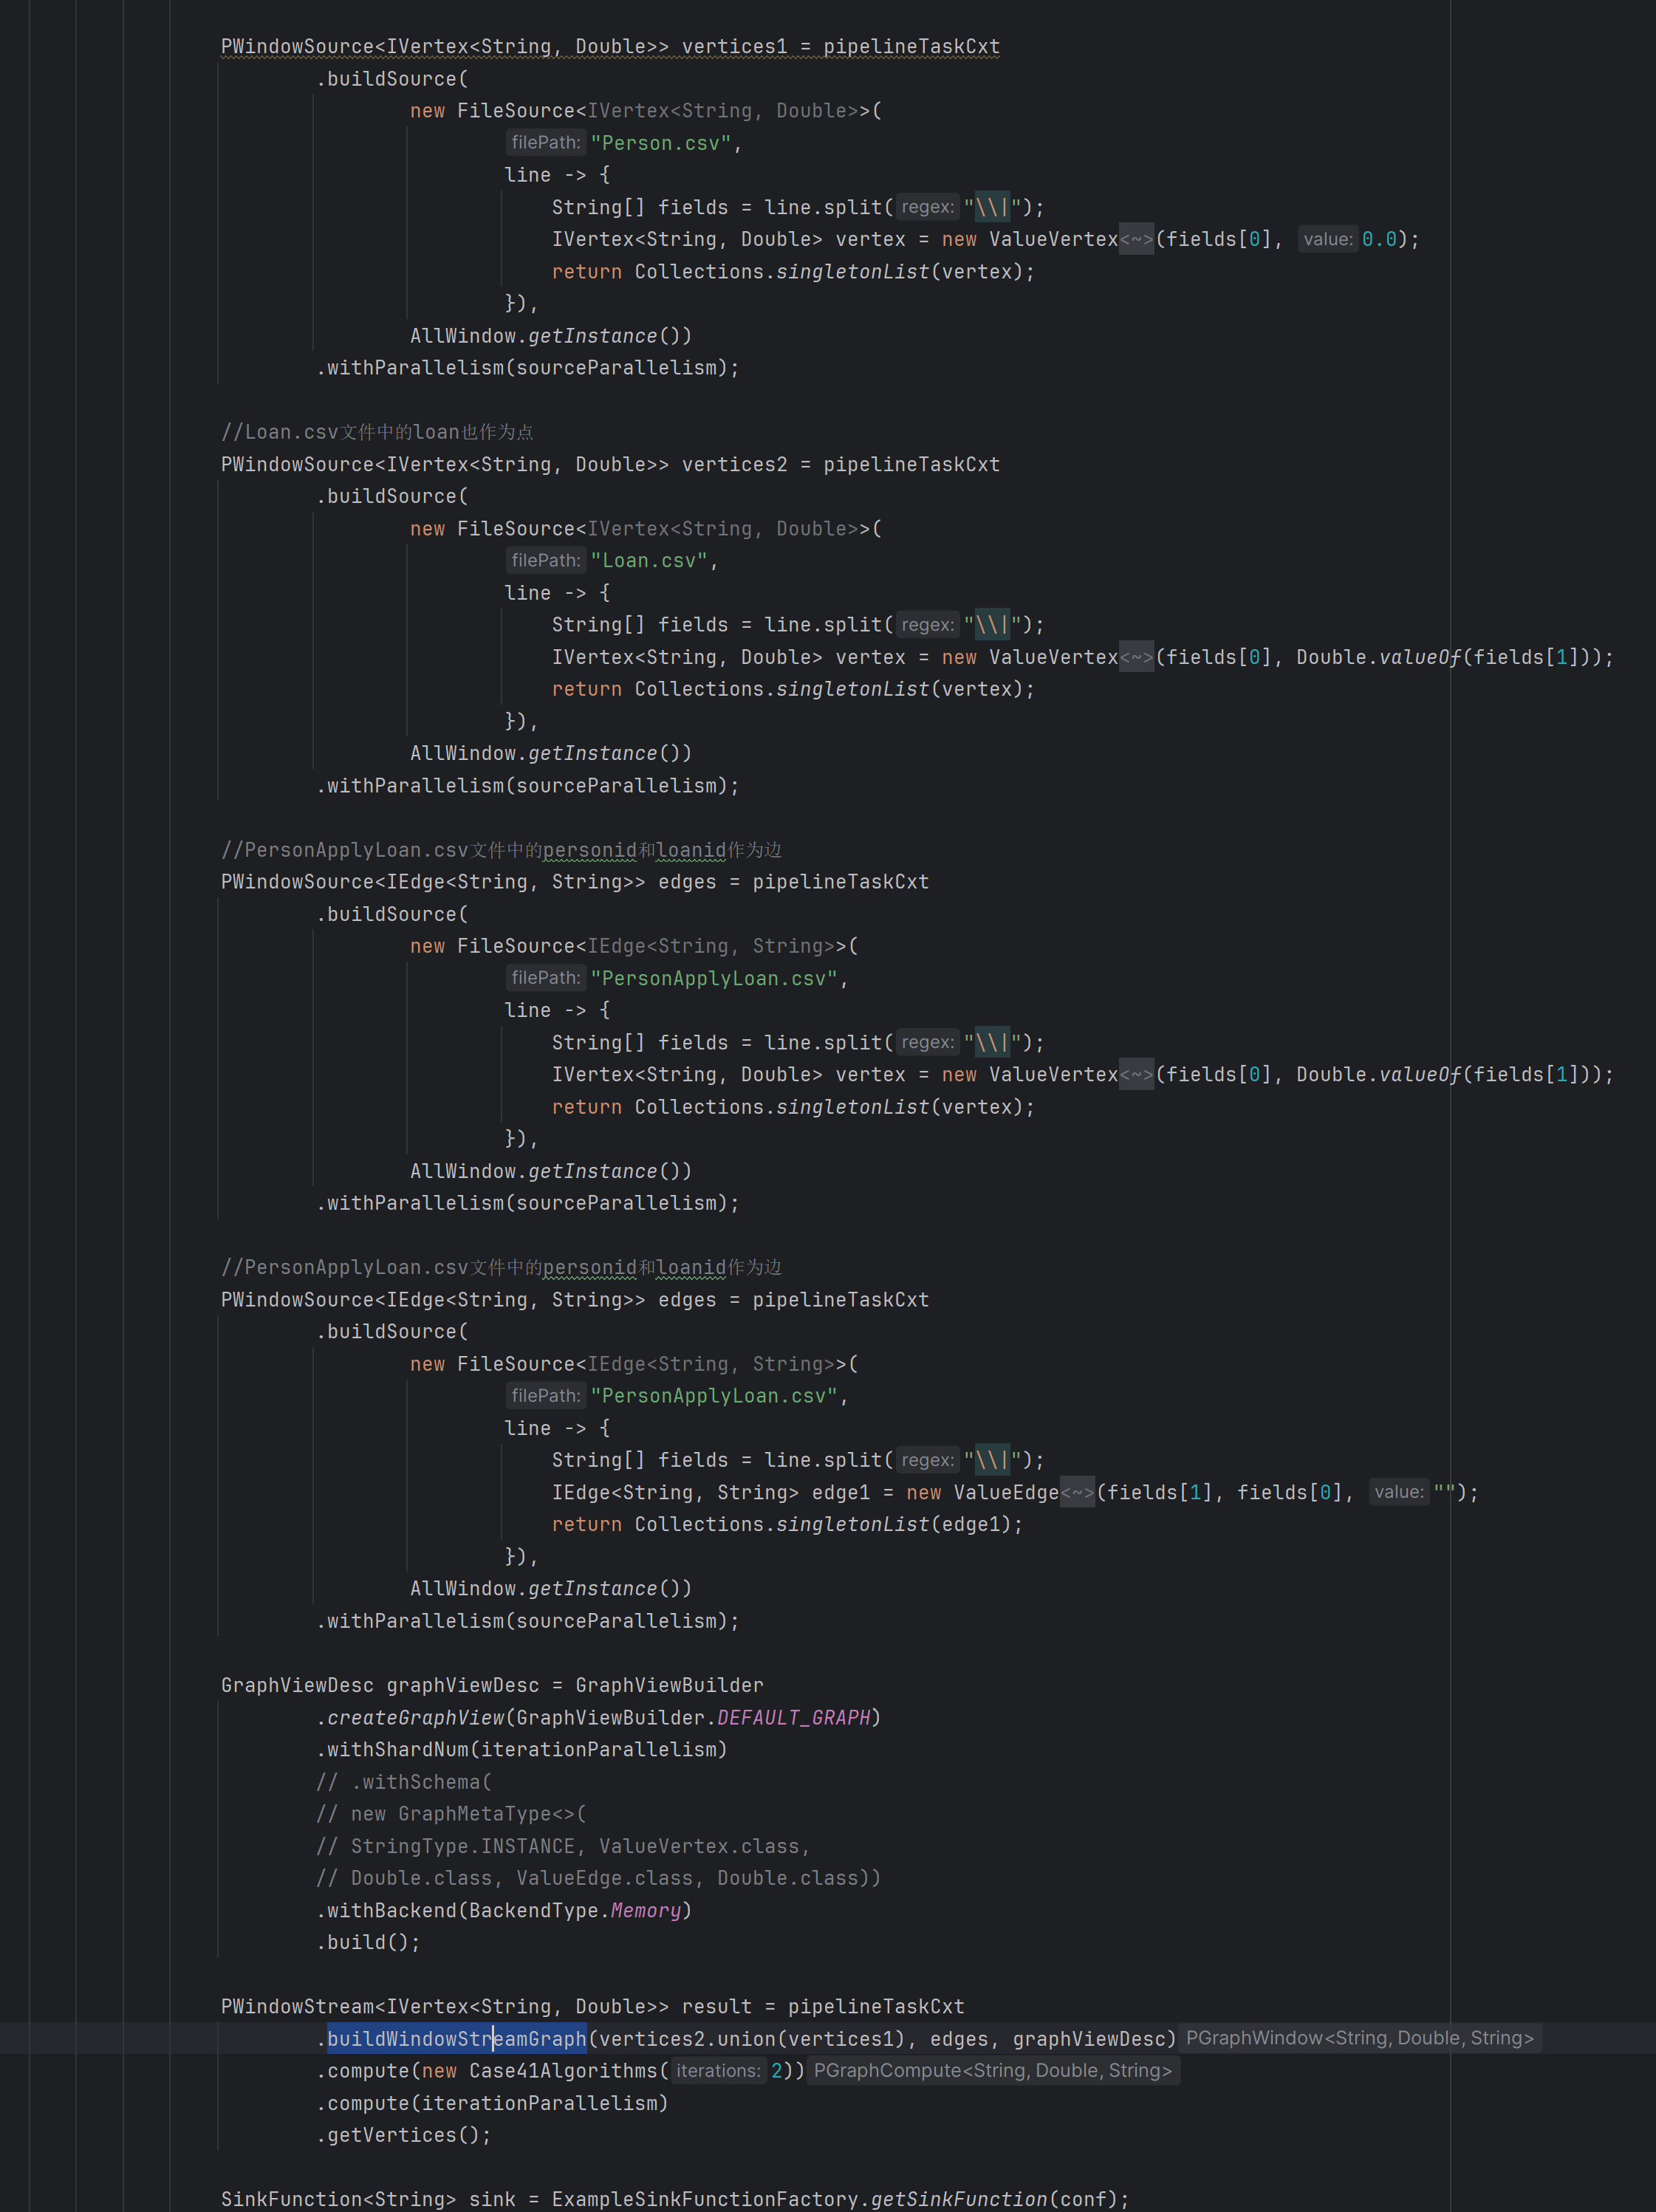
\includegraphics[width=0.85\textwidth,scale=0.7]{./figures/pro3/1.png}
  \end{center}
\end{figure}

接着我们需要得出一个新文件让每个person带上amount,于是,算法思路是进行对所有点
进行两轮迭代,第一轮所有点迭代中,让所有拥有出边的loan点(即此loan有至少一个人
apply),向所有出边的目标点(即person点)发送自己的amount值。最后将自己的value
值设置为 $ -1 $
以方便后续的过滤。(区分person点和loan点的方式是value值是否大于0)

在第二轮迭代中,由于每个点都有一个接收器,我们让所有接收器不为空的点(即person点)
计算接收器的总和 sum 并将 value 值更新为 sum,
到这一步,所有 person 的 value 值 $ >=0 $,所有 loan 的 value 值都为 $ -1 $,
核心代码如下:
\begin{figure}[H]
  \begin{center}
    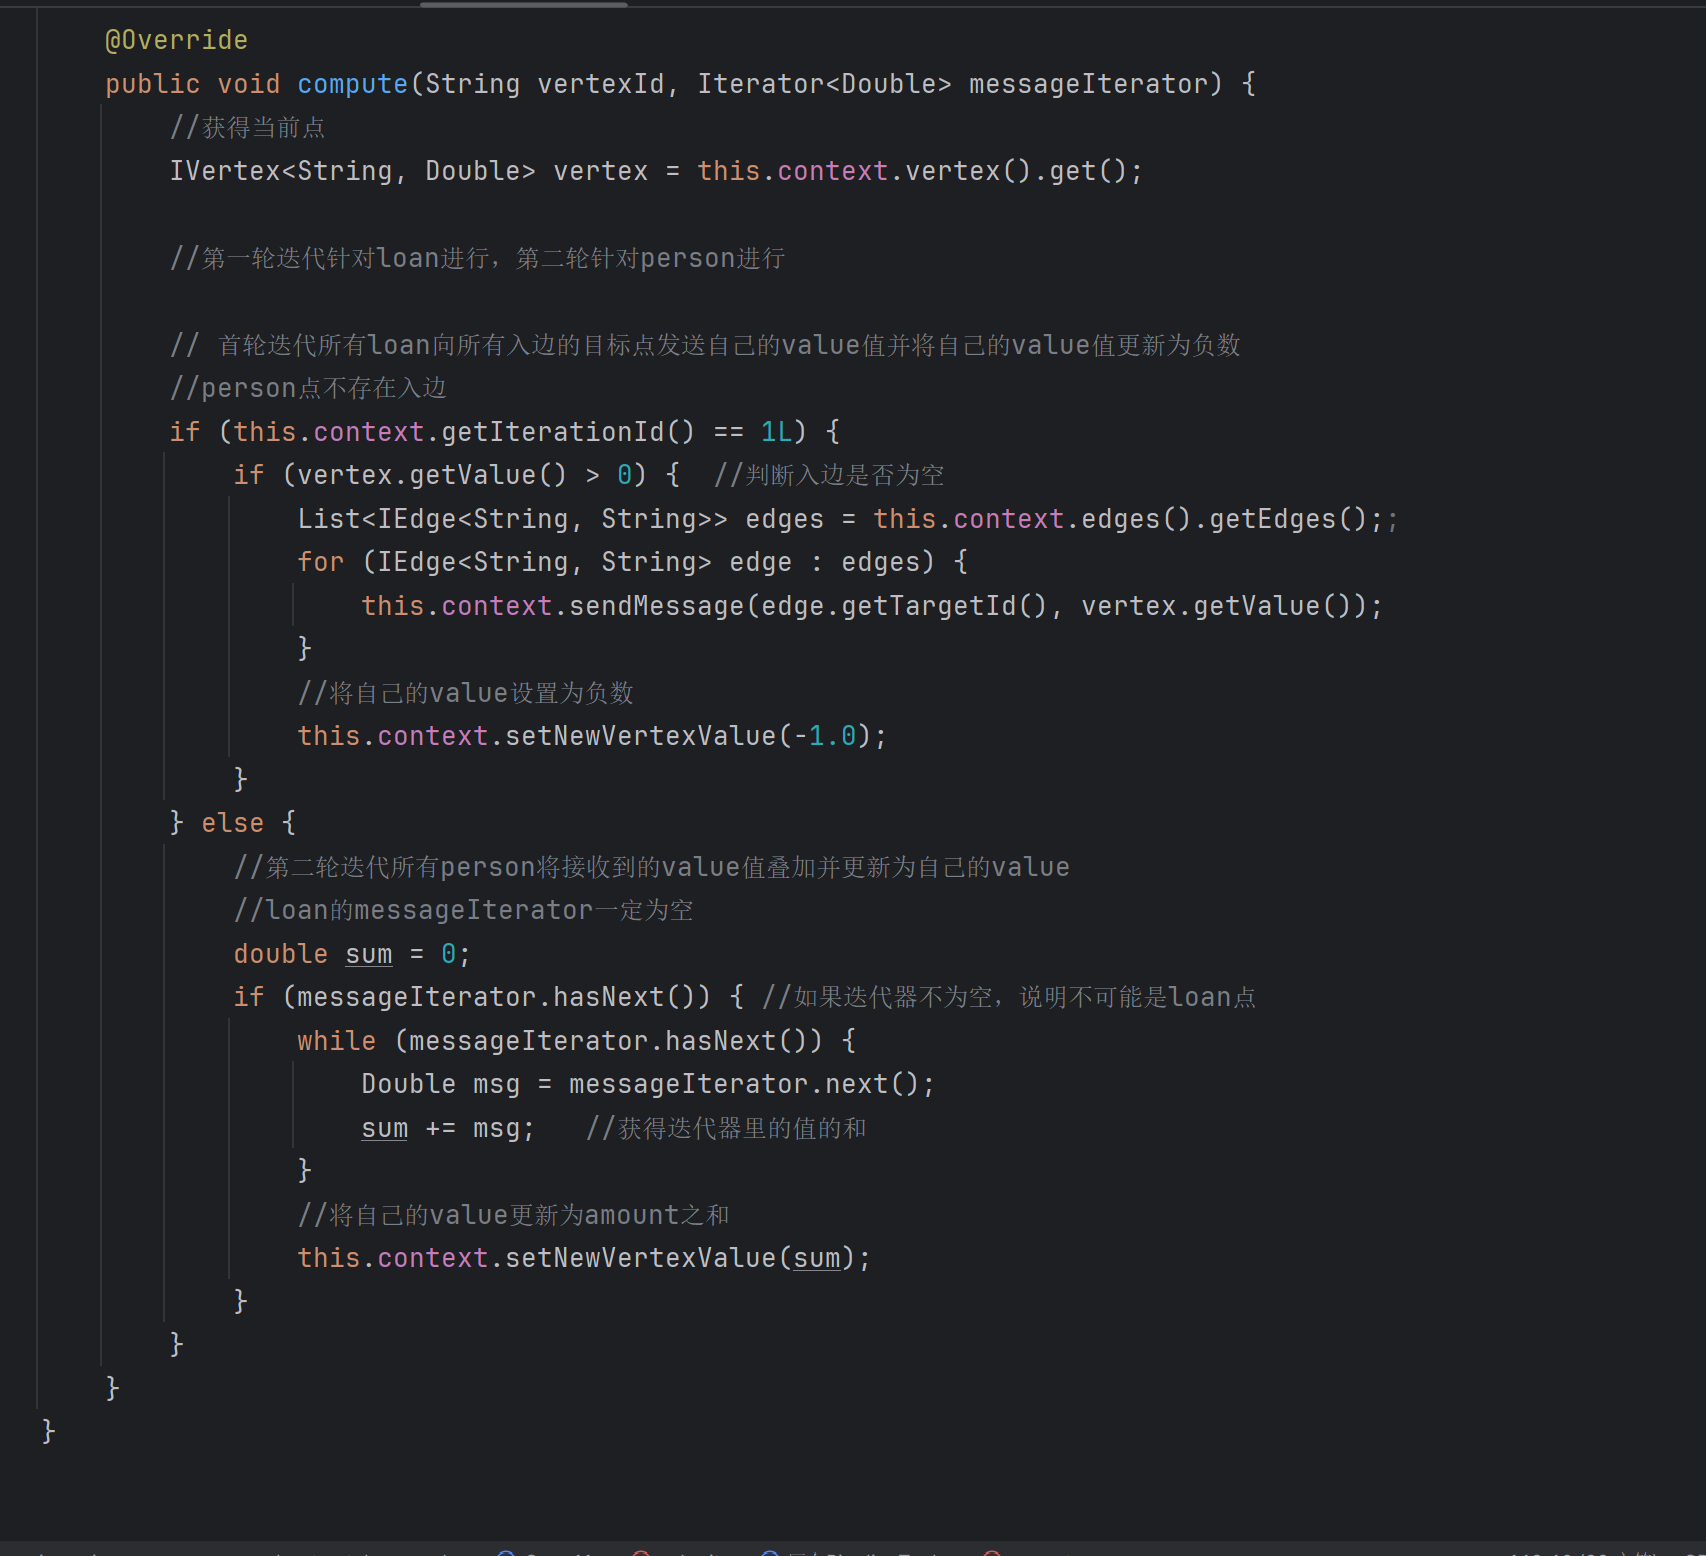
\includegraphics[width=0.85\textwidth,scale=0.7]{./figures/pro3/2.png}
  \end{center}
\end{figure}

最后,将所有点进行过滤涤除value 小于 $ 0 $ 的点(即loan点)得到中间文件。
\begin{figure}[H]
  \begin{center}
    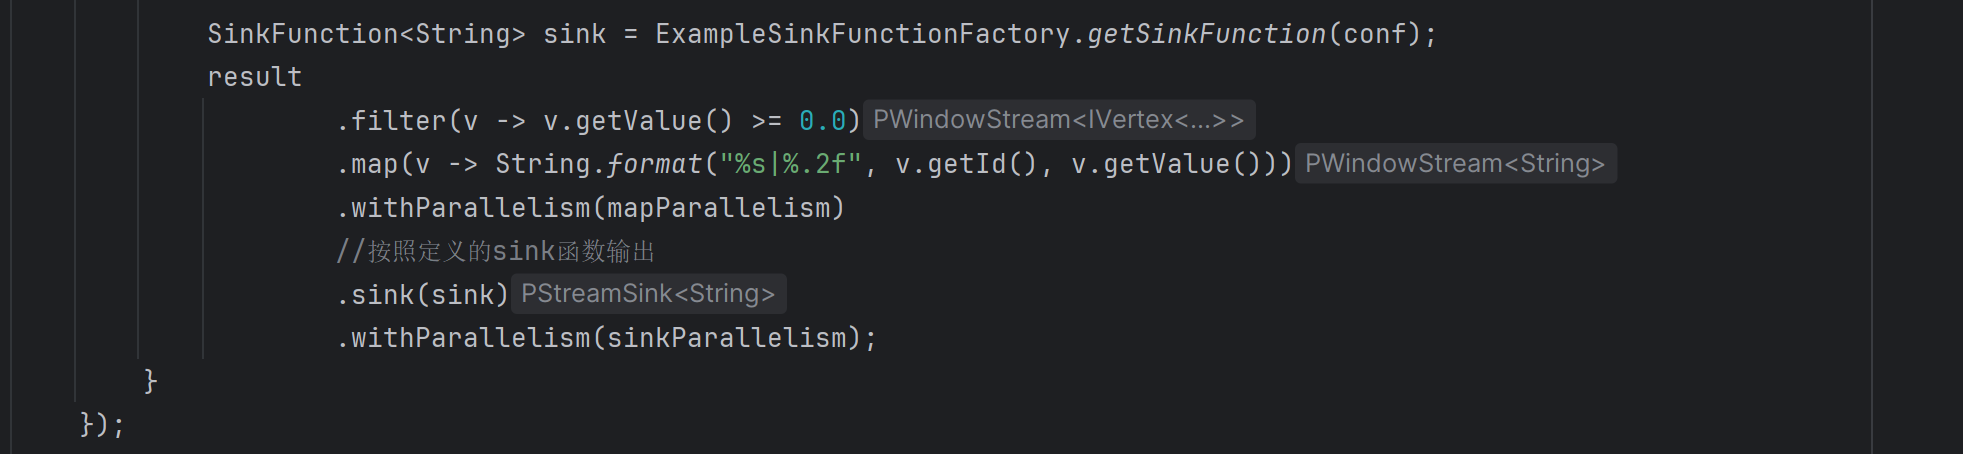
\includegraphics[width=0.85\textwidth,scale=0.7]{./figures/pro3/3.png}
  \end{center}
\end{figure}

接着进入第二步操作,首先因为我们要将中间文件与personguaranteeperson文件联合起来
构建成图,点的id为person的id,点的value为person的value,边的value为空字符串:
\begin{figure}[H]
  \begin{center}
    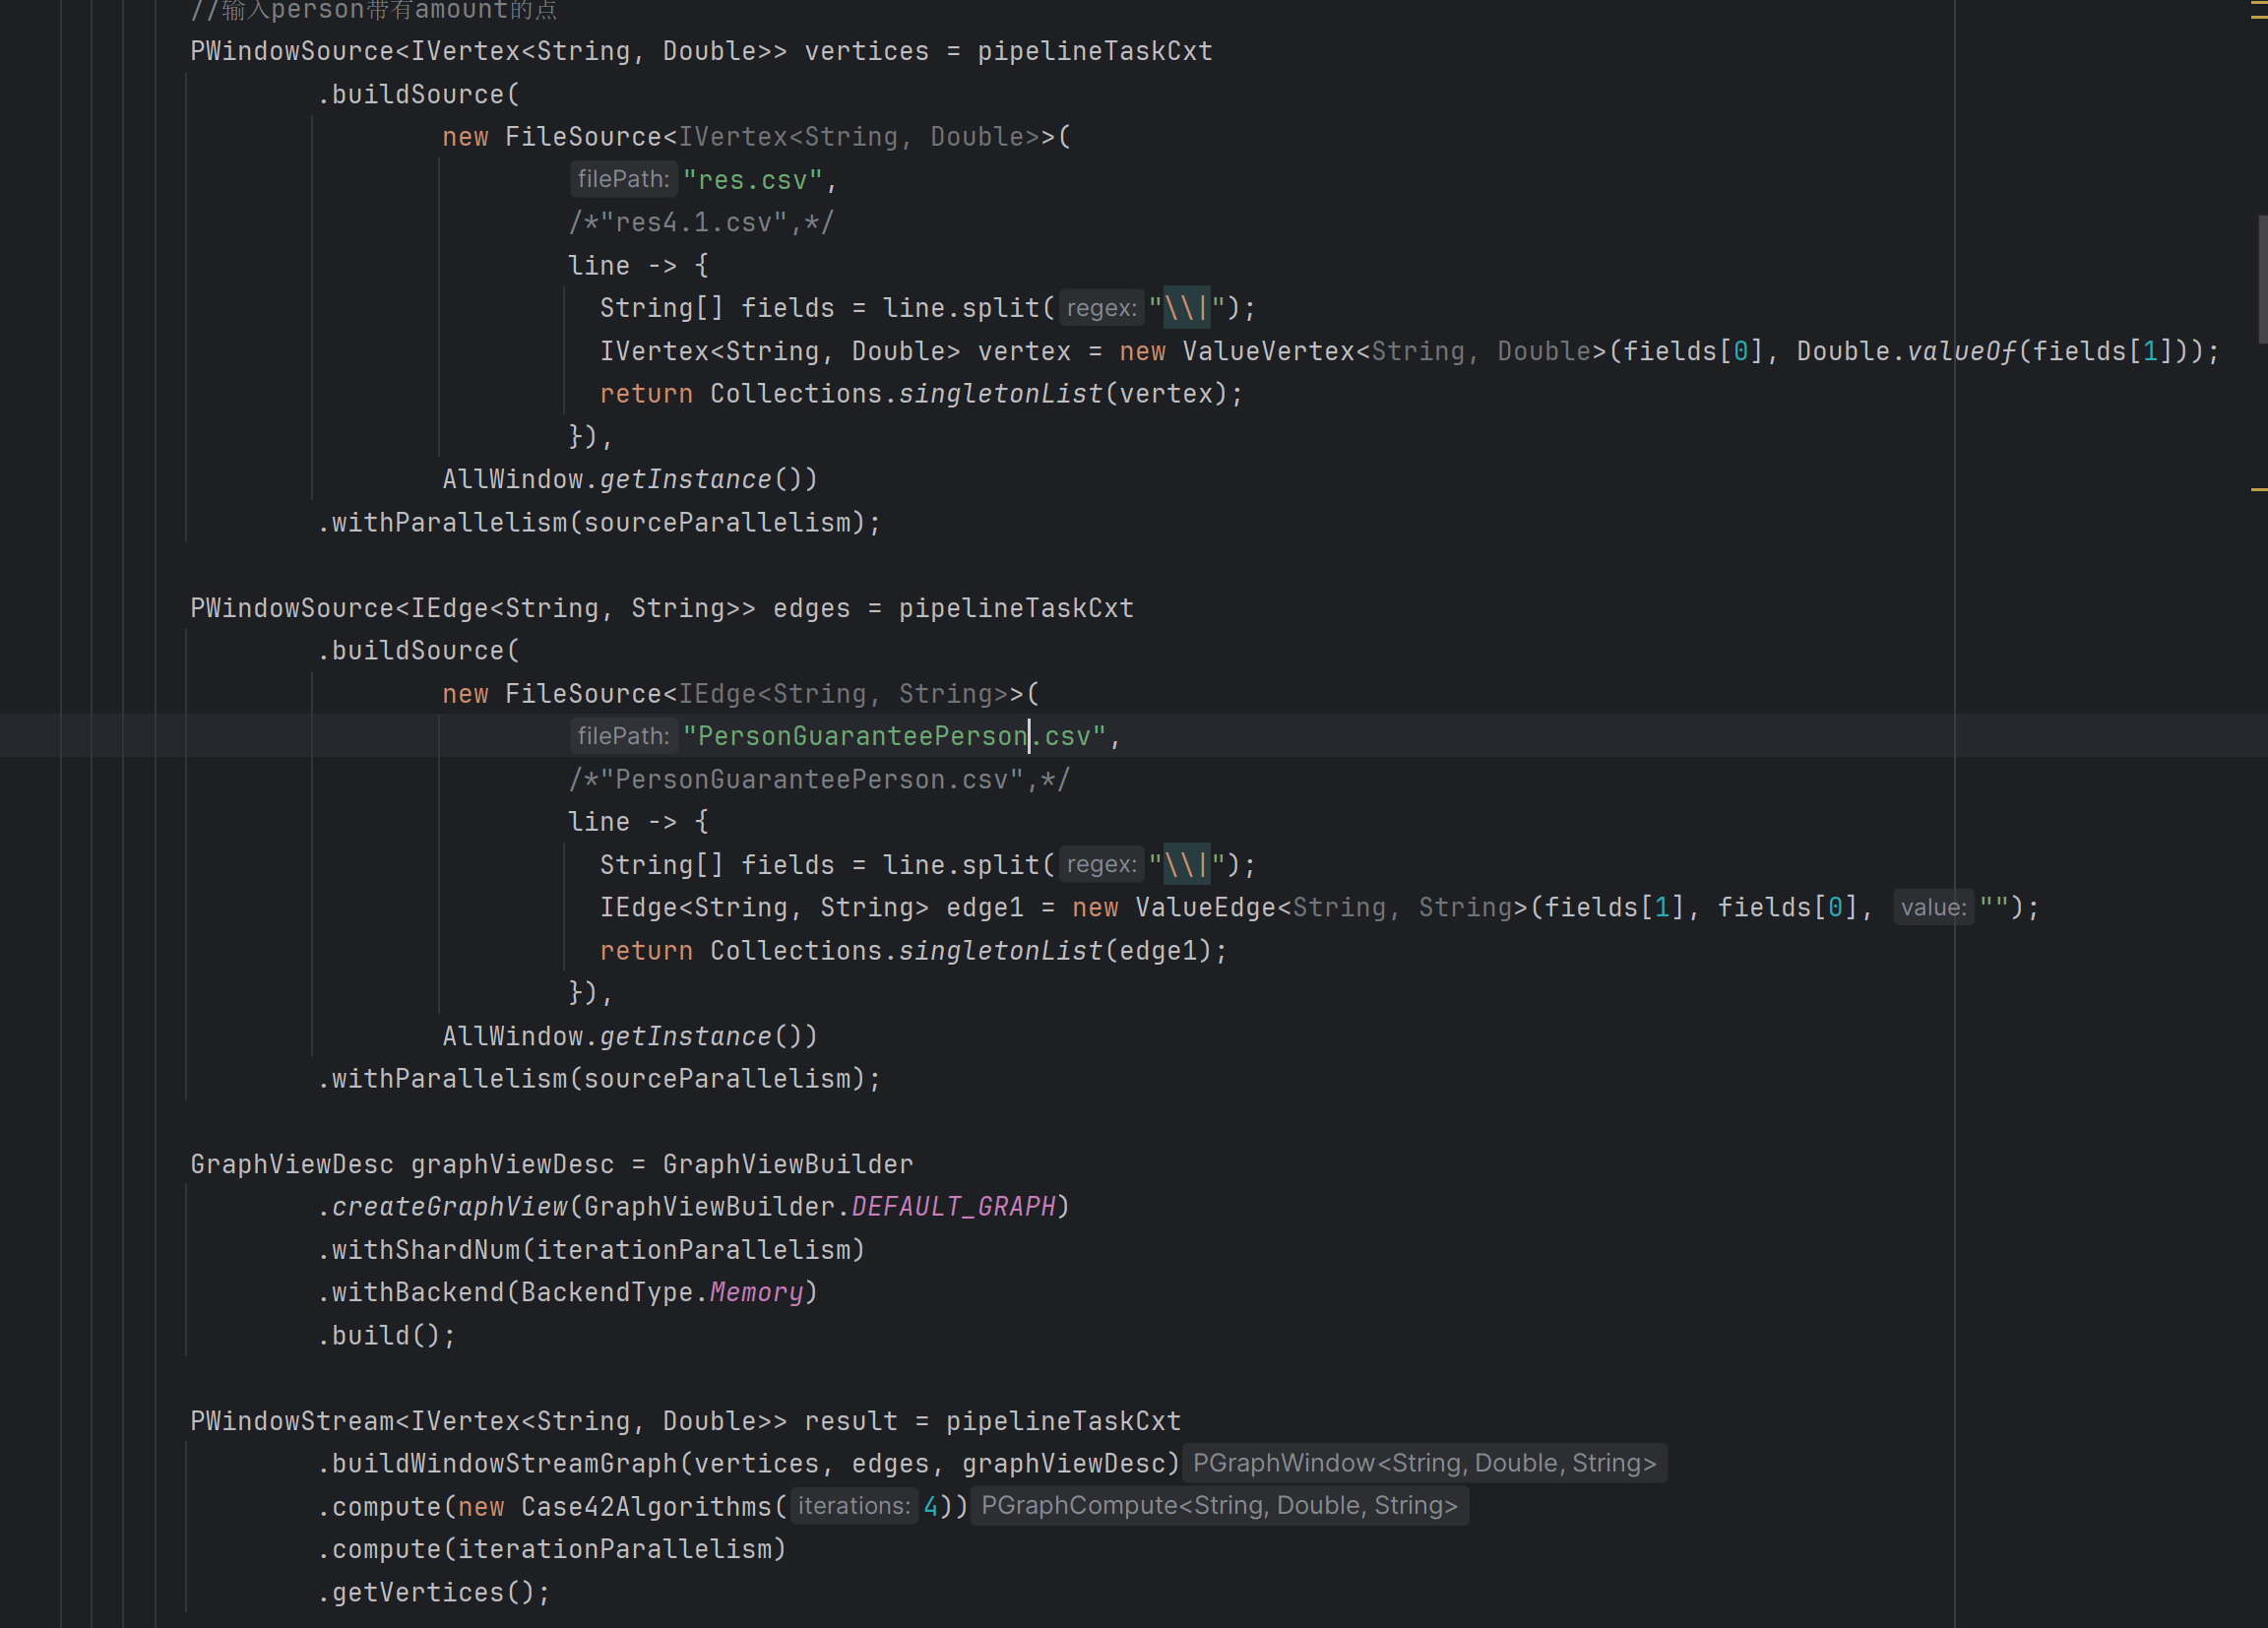
\includegraphics[width=0.85\textwidth,scale=0.7]{./figures/pro3/4.png}
  \end{center}
\end{figure}

接着我们进行四轮迭代,核心思想是在第n轮迭代中,所有点的value值都用来存储其下n-1
级所有点的amount总和。第一轮迭代中,所有点向它的所有出边目标点发送自己的value
值即amount值,在第二轮迭代中让点计算接收器的值sum并将value值更新为sum,同时继
续向此点的所有出边点发送自己的value值,在第二轮迭代完成后每一个点的value值都是
其下一级所有点的amount总和。在第三轮迭代中所有点计算接收器中的总和sum,接着继
续向所有出边点发送sum,同时更新自己的value值为sum+value。第三轮迭代结束后所有
点的value值即为其下两级所有点的amount总和。在第四轮迭代中所有点重复第三轮迭代
的更新操作并得到最终结果。
需要注意的是,接收器每一轮都会进行更新,只存储新的接收值,同时,接收器没接收信
息的点将不会进入下一轮迭代,这就是为什么在下面代码中我们让所有点都向自己的接收
器发送 $ 0.0 $(不影响结果)。核心代码如下:
\begin{figure}[H]
  \begin{center}
    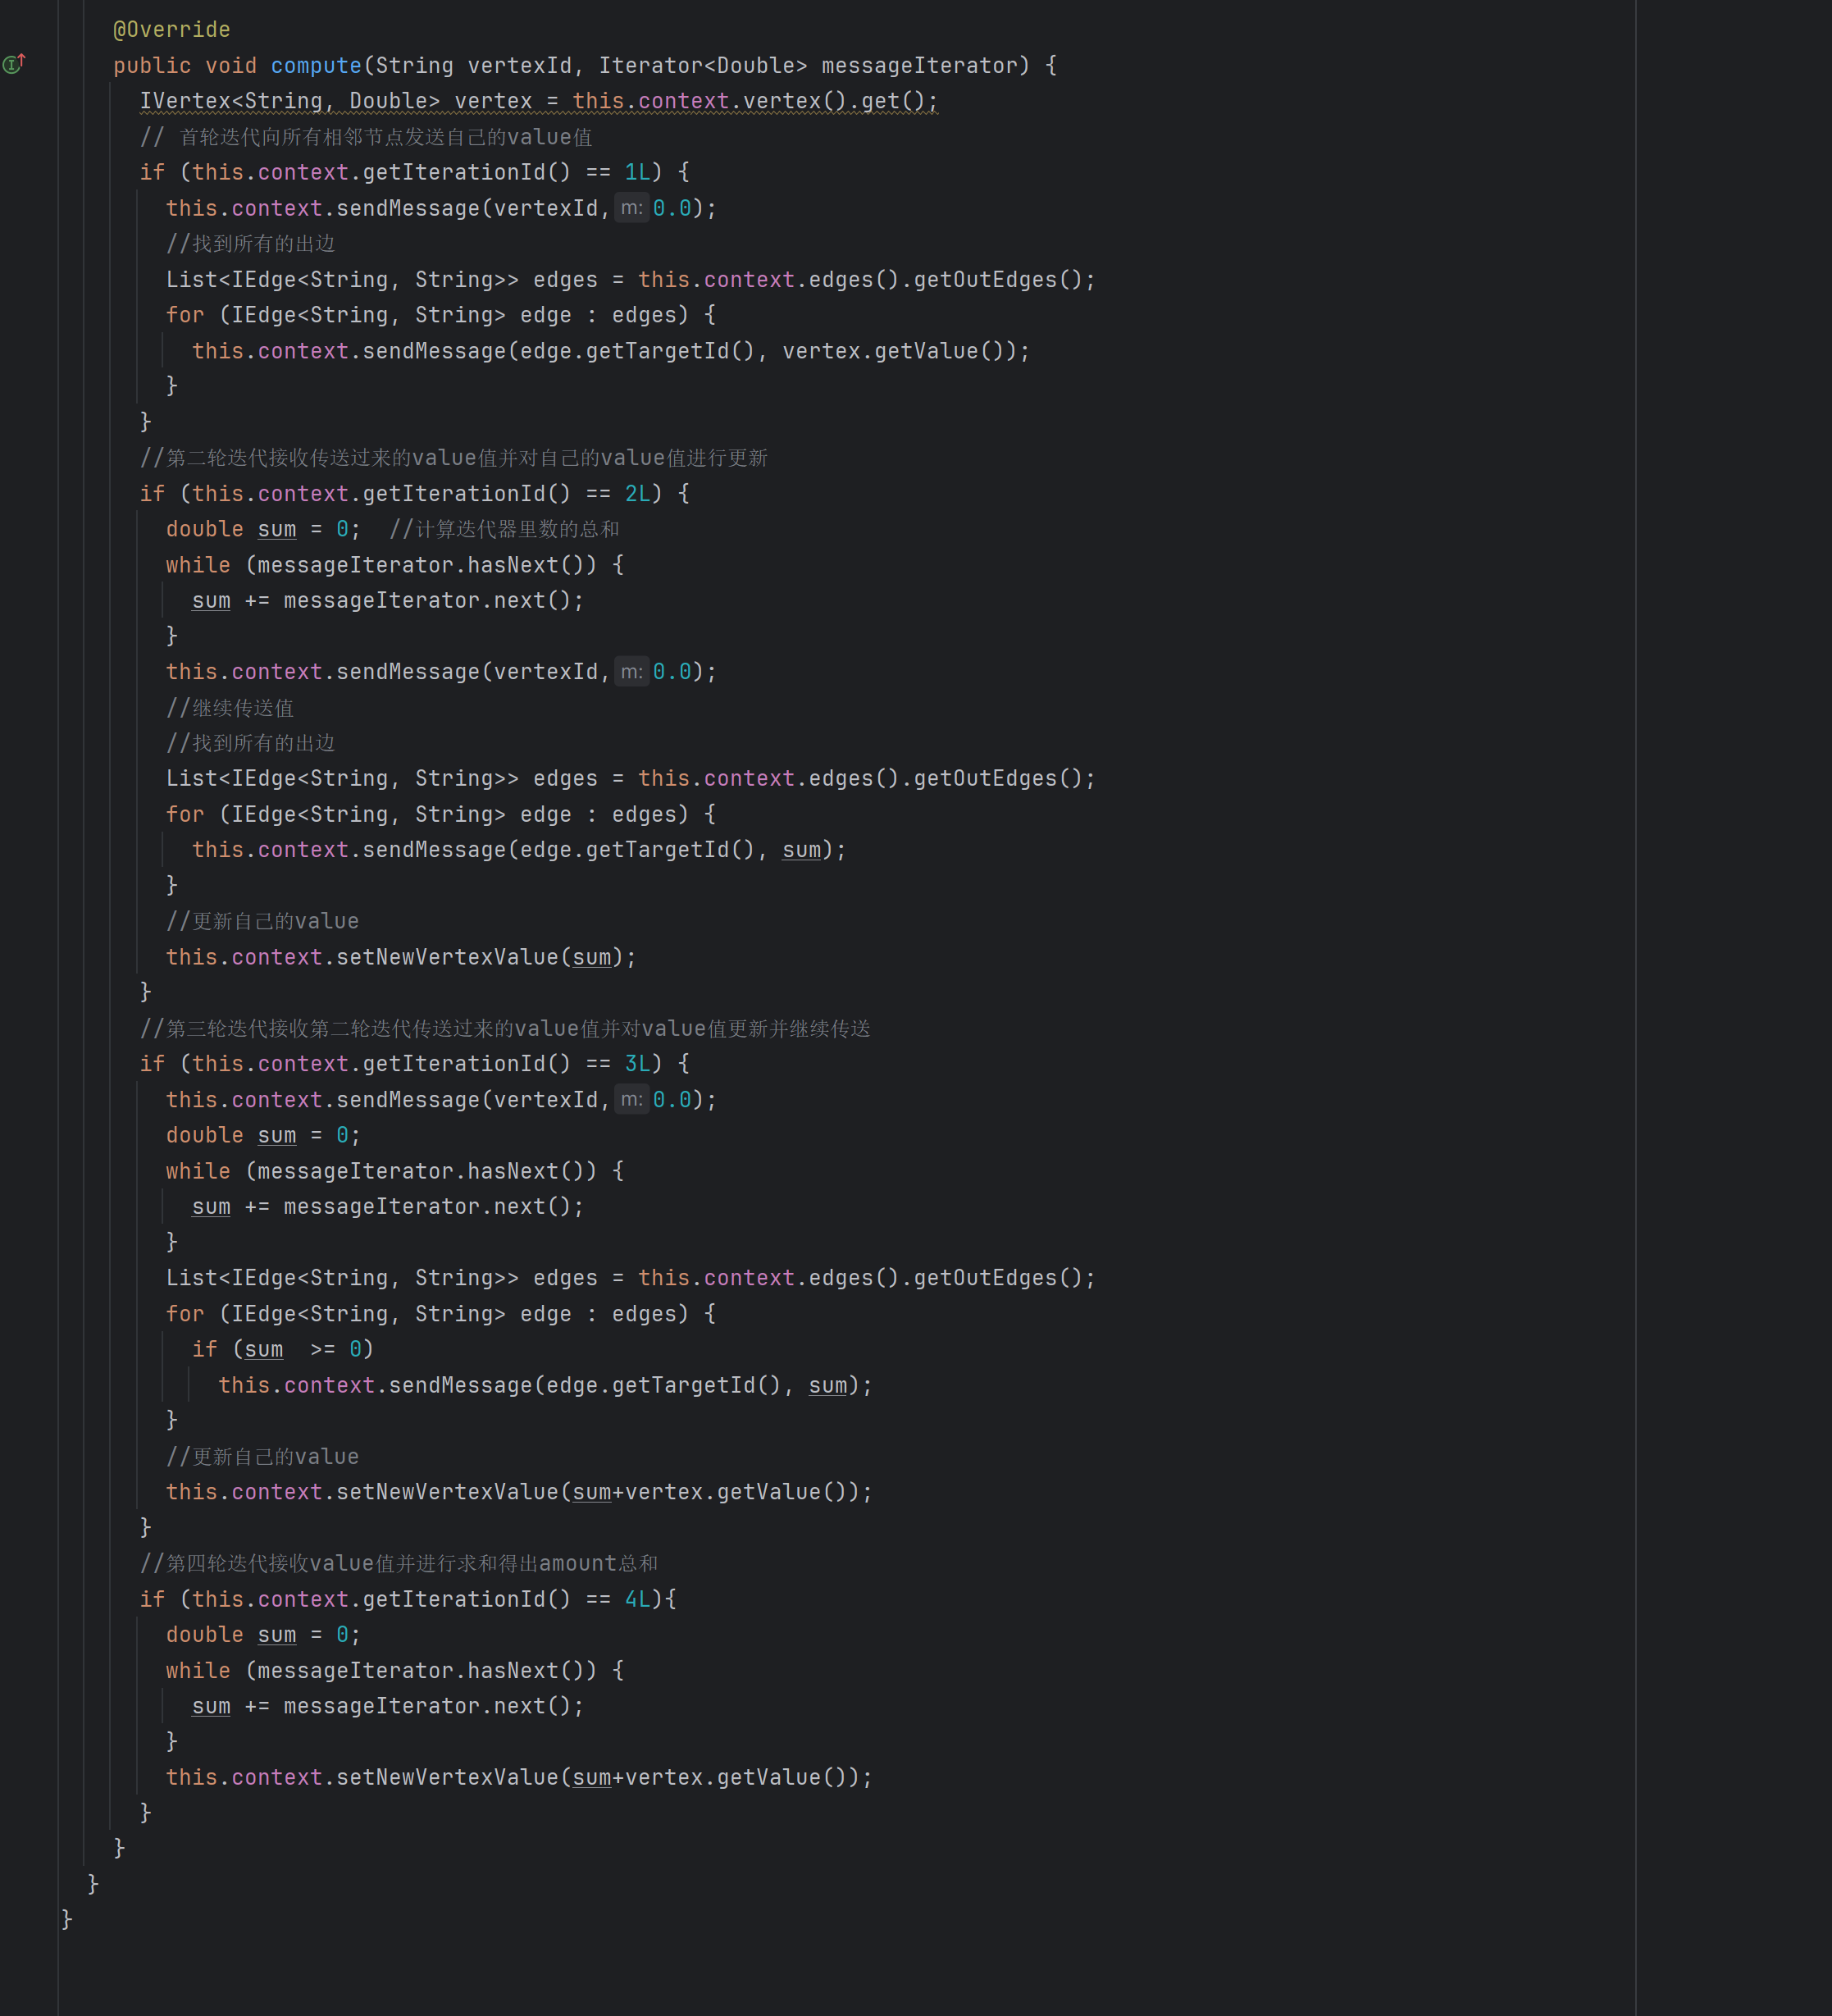
\includegraphics[width=0.85\textwidth,scale=0.7]{./figures/pro3/5.png}
  \end{center}
\end{figure}

最后将结果保存到文件中
\begin{figure}[H]
  \begin{center}
    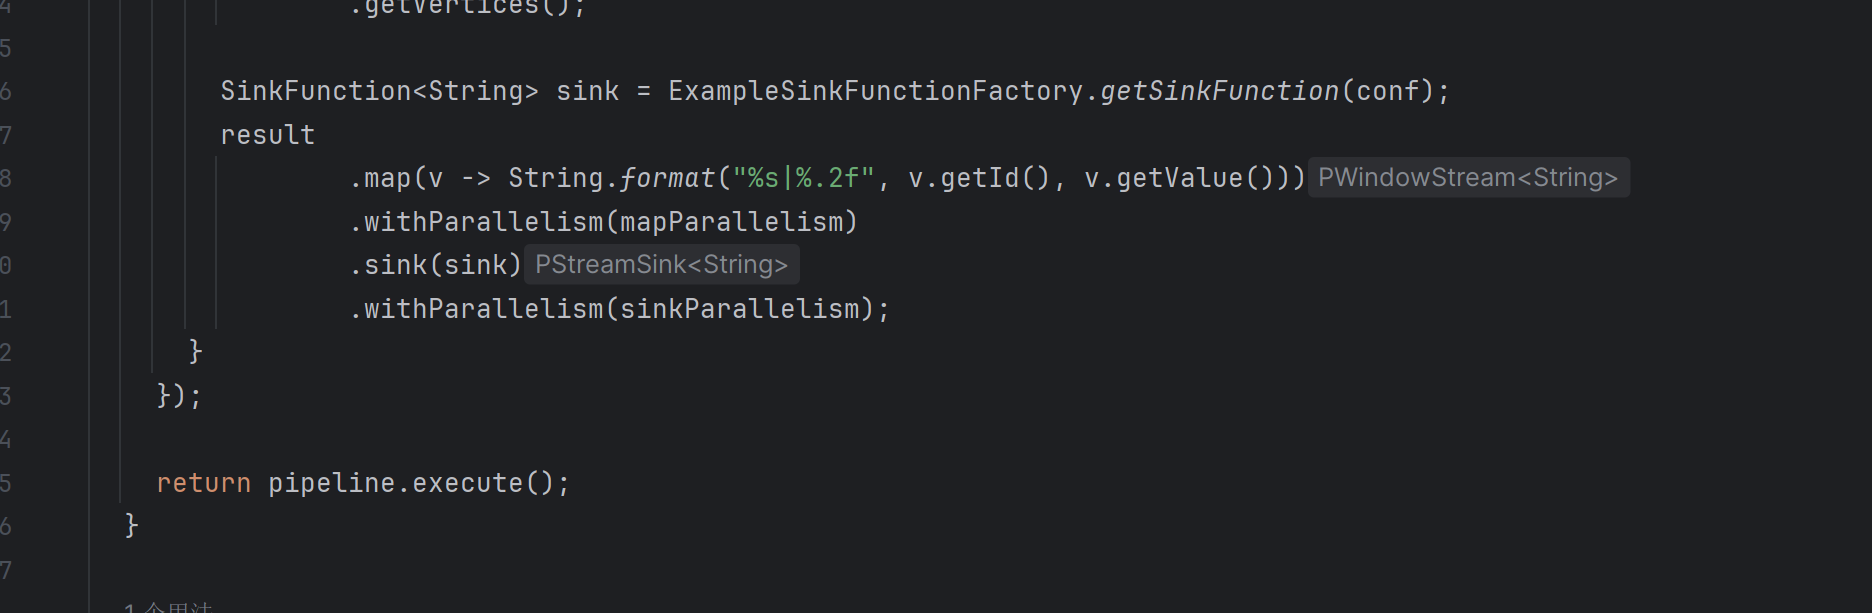
\includegraphics[width=0.85\textwidth,scale=0.7]{./figures/pro3/6.png}
  \end{center}
\end{figure}

但是,提交结果以失败告终了,经过分析,我们发现这个算法不能处理环的问题,因为如
果图中存在环,那么有的点的value值就会就会计算两遍。

\subsubsection{尝试代码优化改进}
上面的算法存在问题,所有我们进行思考后,决定改进第二步操作的compute算法,我们
将点封装成对象,并在迭代中将传递的数据类型改为string类型,可以来判断发送点的具体
信息,用set可以进行点的去重,判断发送源点是否已经给自己发送过数据。每个点首轮
向邻居发送一个消息(点id,1,0.00),当一个点收到消息后若消息的第二个元素
为1或2则直接给消息第一个元素对应的点发送自己的value并将第二个元素加1
传递给邻居;若第二个元素为3,则发送value而不继续传递;最后第二个元素
为4的就是担保链上所有的点发来的消息。
点的类描述如下:
\begin{figure}[H]
  \begin{center}
    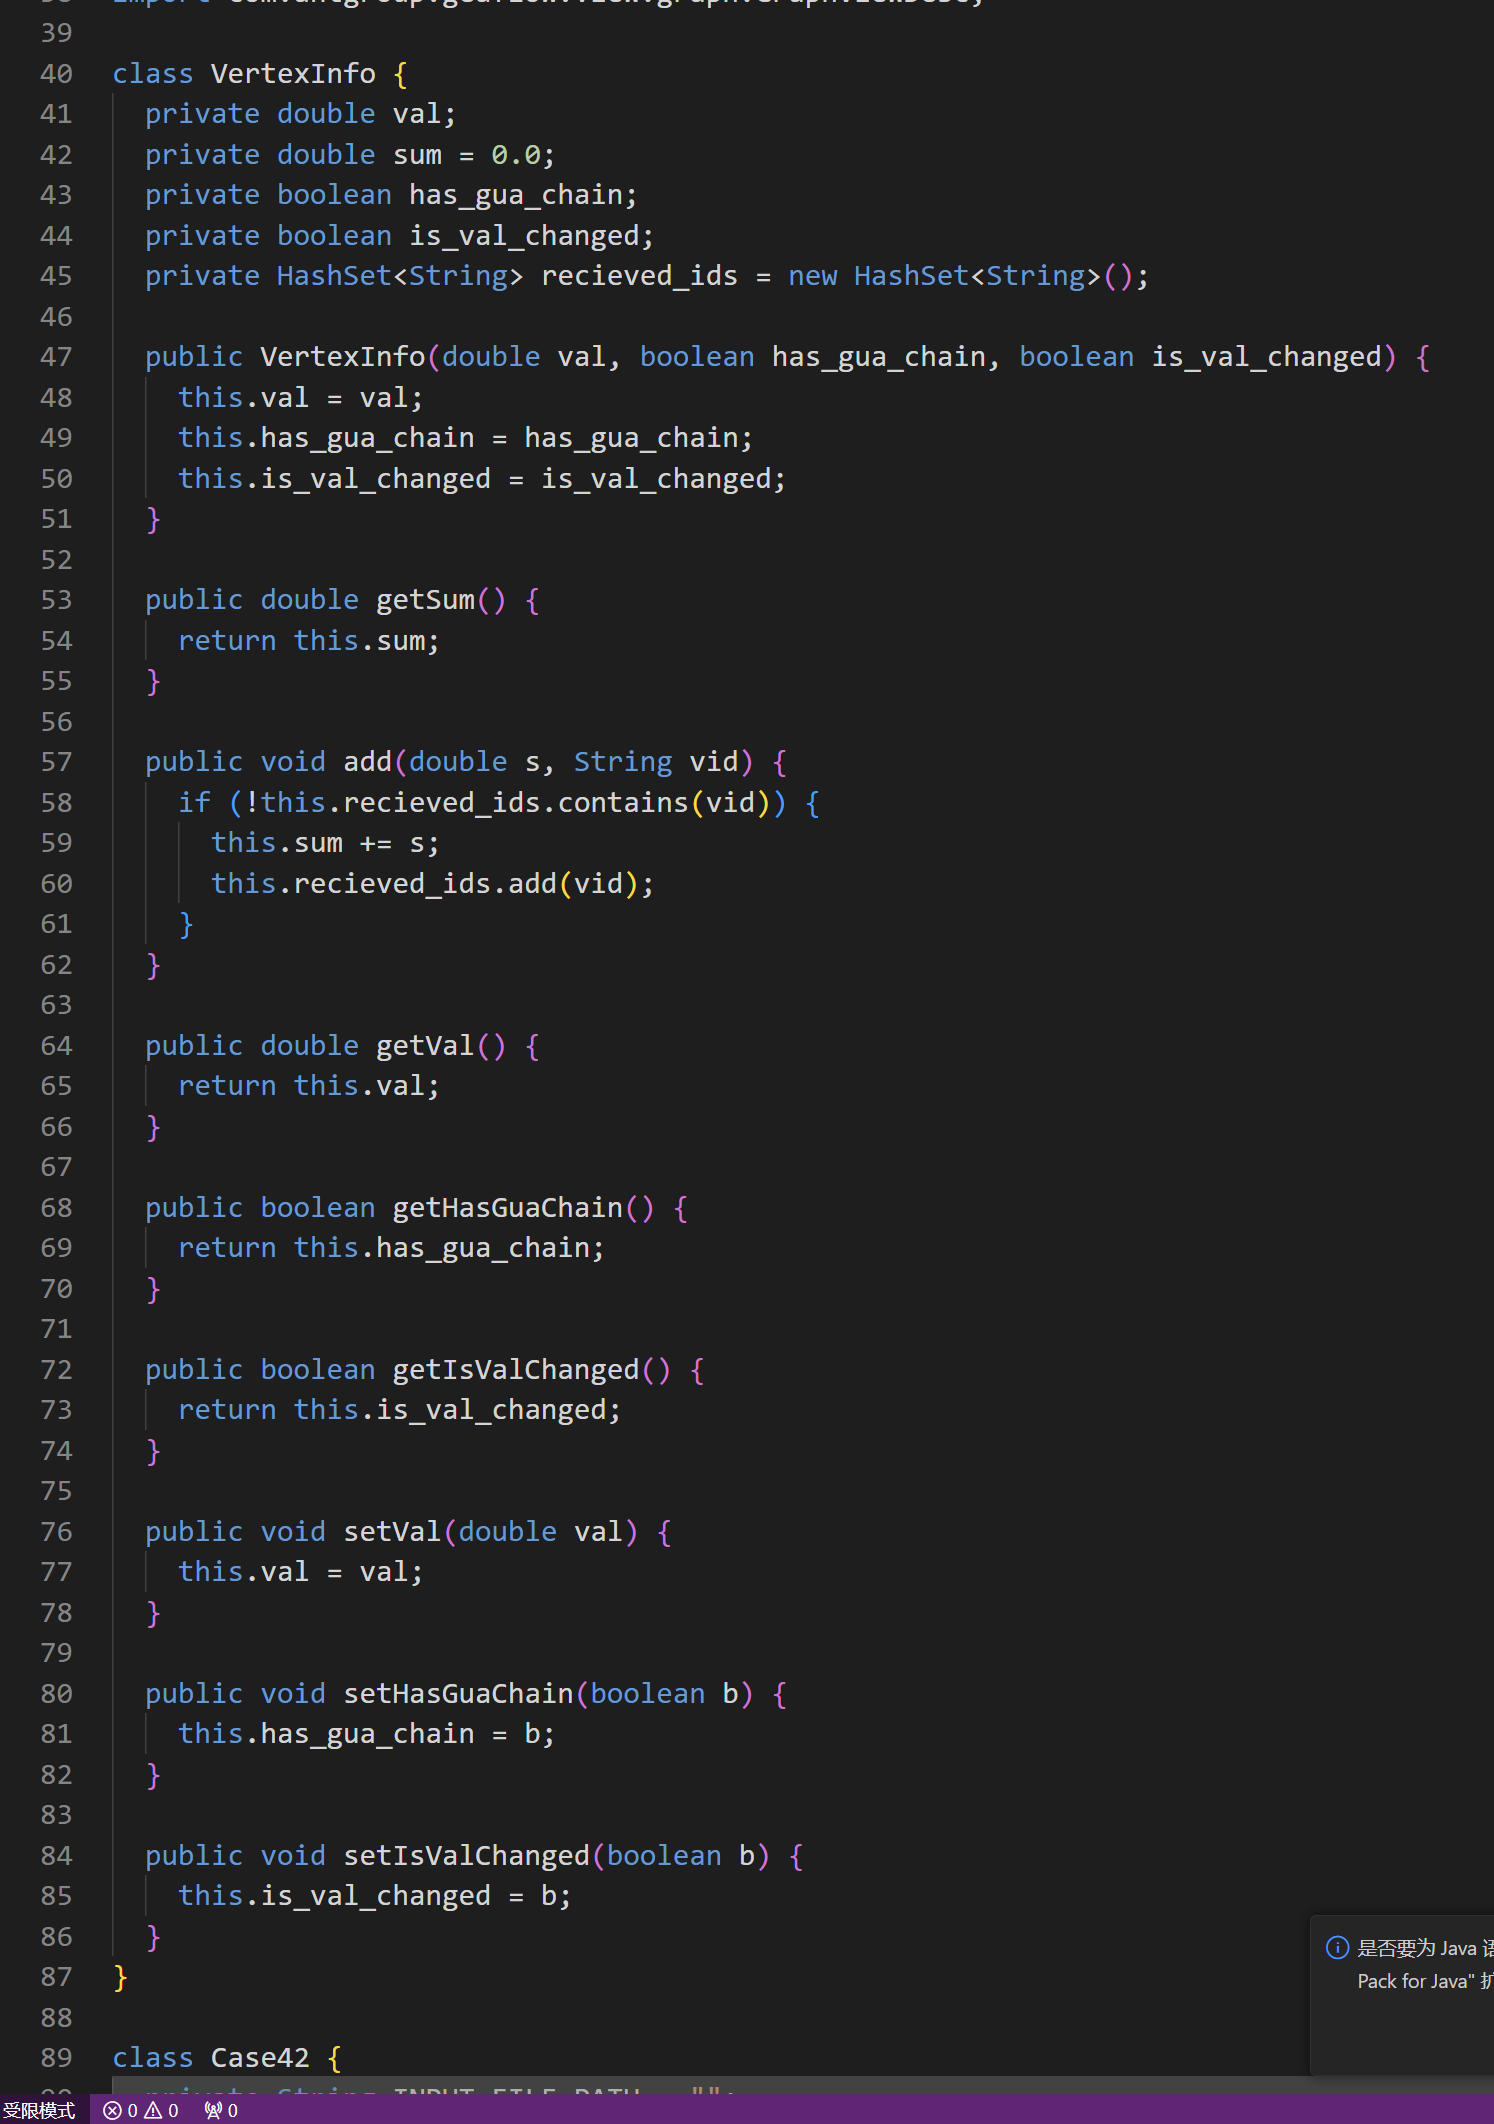
\includegraphics[width=0.85\textwidth,scale=0.7]{./figures/pro3/7.png}
  \end{center}
\end{figure}

更新后的compute如下:
\newpage

\begin{figure}[H]
  \begin{center}
    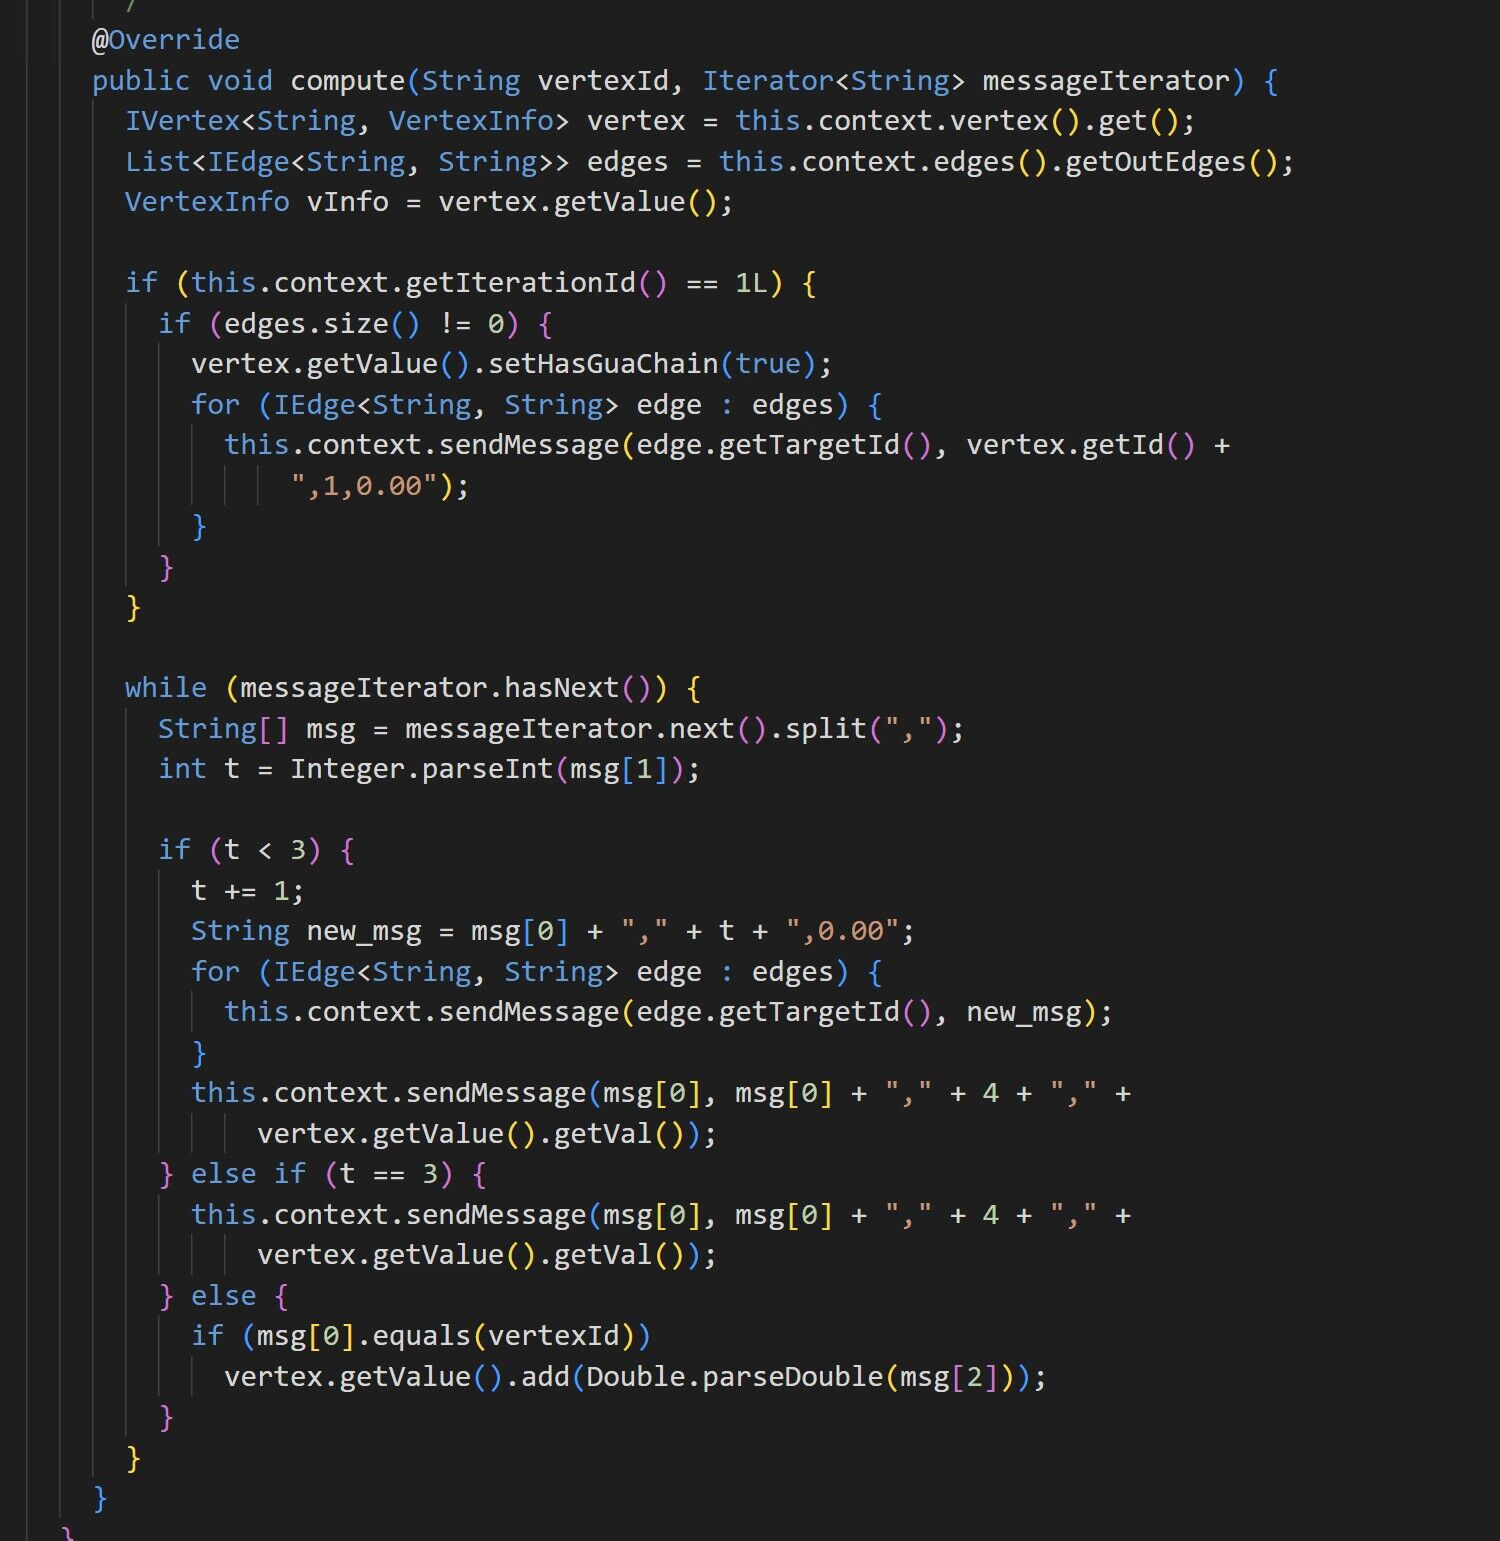
\includegraphics[width=0.55\textwidth,scale=0.5]{./figures/pro3/8.png}
  \end{center}
\end{figure}

我们尝试自己创建文件将自己能想到的所有情况进行测试,结果均正确。但是依然过不了
测试,宣告本题以失败告终。但是在尝试过程中也收获了许多知识点。

\subsection{个人贷款统计问题}
具体问题描述可见 \ref{pro4} 个人贷款统计问题一节.

备注:此case1我们花了一定时间,没有通过评测。最初其结果集有误,后续赛事组才进行
修改,我们当时忙于处理case4,遂对该题没有过多的深入。

此问题涉及的数据文件有:
\begin{itemize}
  \item Person.csv(点)
  \item Account.csv(点)
  \item Loan.csv(点)
  \item AccountTransferAccount.csv(边)
  \item LoanDepositAccount.csv(边)
  \item PersonOwnAccount.csv(边)
\end{itemize}

\subsubsection{思路历程}
根据题目需分三步走,逐步将loan值往前传。首先导入account点和loan点,
通过loandepositaccount的边和其值amout创建一张图,向前传递amount值;再将上一步
生成的含有accountid和value的表与accounttransferaccount的边结合生成一张图,将value
的值向前传递;最后将上一步生成的含有accountid和value的表与personownaccount边、
person点相结合,向前传递value值实现个人贷款的汇总。

\subsubsection{代码分析与实现}
运用赛题所给的接口,我们先将account和loan都当作点,点的id即为account或loan对应
的id,将account的初始value设为0,将loan的初始value设为-1(方便后续筛选);而对
于边,我们将loandepositaccount的amount设为其边的value,两侧点按顺序填入相应的id,
通过输入流pwindowsource分别进行输入。接着我们用buildwindowstreamgraph进行构图,
在构图中我们用union操作将loan和account点合并在一起。考虑到loan和account的id有重
复的部分(通过set检测,遍历两个文件后统计数量是否变化),由于loan点在后续代码中
并没有使用,因此在loan点的id前加入字符“l”以进行区分,防止account之间或者loan
之间的相连。代码如下:
\begin{figure}[H]
  \begin{center}
    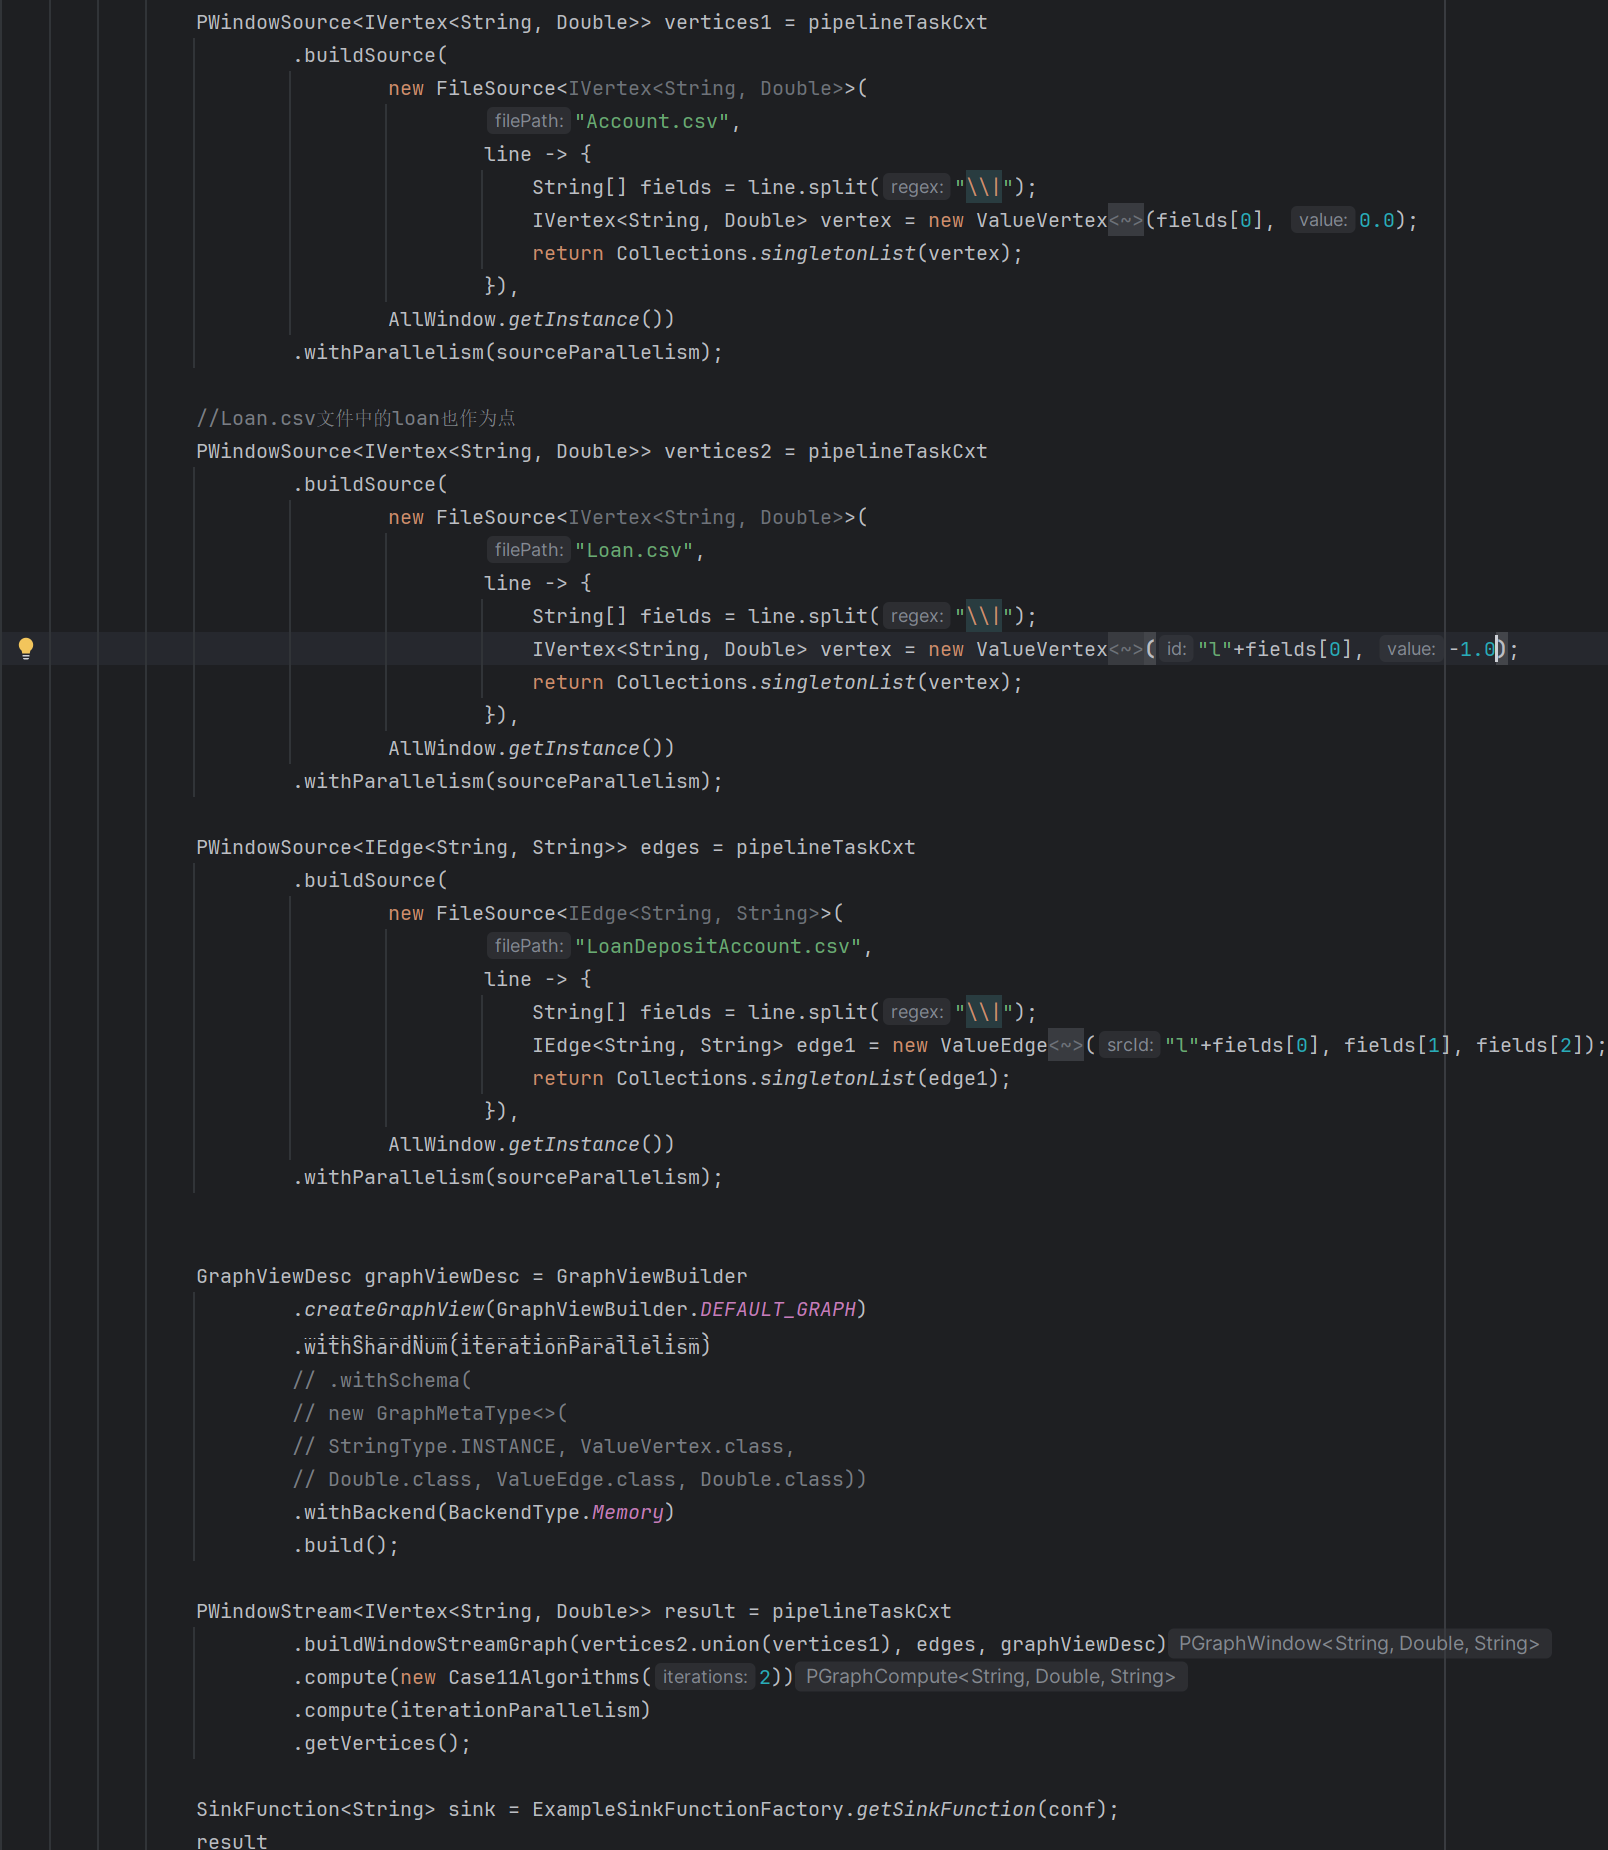
\includegraphics[width=0.85\textwidth,scale=0.7]{./figures/pro4/1.png}
  \end{center}
\end{figure}

接着我们需要得出一个新文件让每个account带上amount,于是,算法思路是进行对所有
点进行两轮迭代,第一轮所有点迭代中,让所有拥有出边的loan点(即此loan有至少一个
账户deposit),向所有出边的目标点(即account点)发送边的amount值。在第二轮迭代
中,由于每个点都有一个接收器,我们让所有接收器不为空的点计算接收器的总和sum并
将value值更新为sum,
到这一步,所有account的value值大于等于 $ 0 $,所有loan的value值都为 $ -1 $,核心代码如下:
\begin{figure}[H]
  \begin{center}
    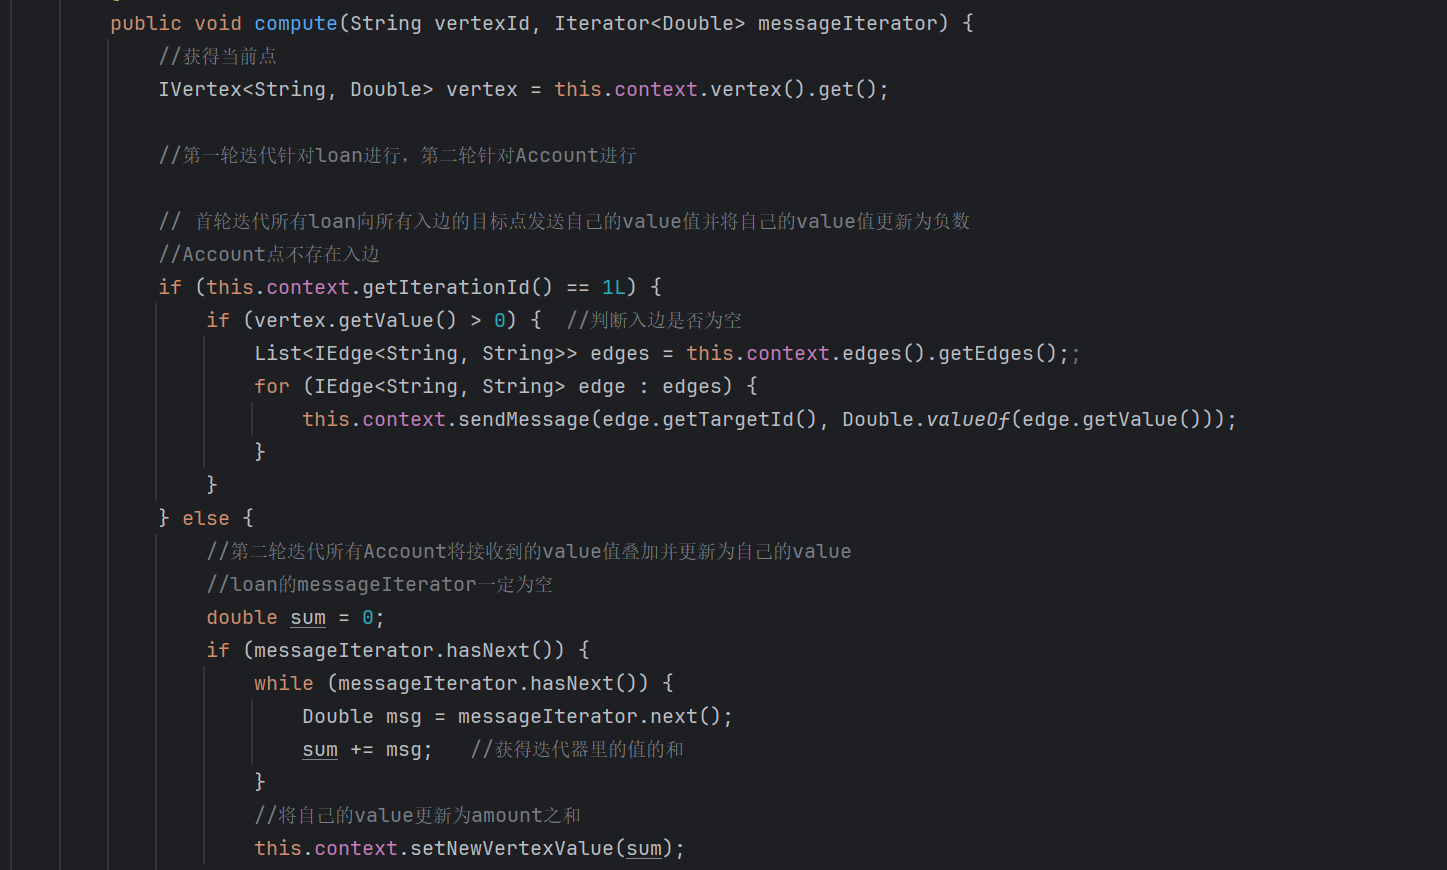
\includegraphics[width=0.85\textwidth,scale=0.7]{./figures/pro4/2.png}
  \end{center}
\end{figure}

最后,将所有点进行过滤涤除value 小于 $ 0 $ 的点(即loan点)得到中间文件。
\begin{figure}[H]
  \begin{center}
    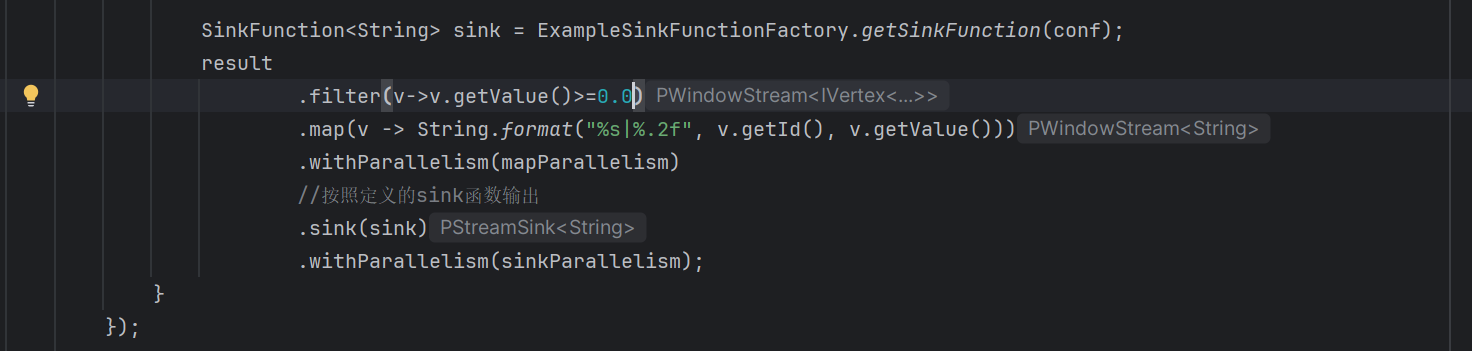
\includegraphics[width=0.85\textwidth,scale=0.7]{./figures/pro4/3.png}
  \end{center}
\end{figure}

接着进入第二步操作,首先我们将中间文件与accounttransferaccount文件联合起来构建成
图,点的id为account的id,点的value为account的value,边的value为空字符串:
\begin{figure}[H]
  \begin{center}
    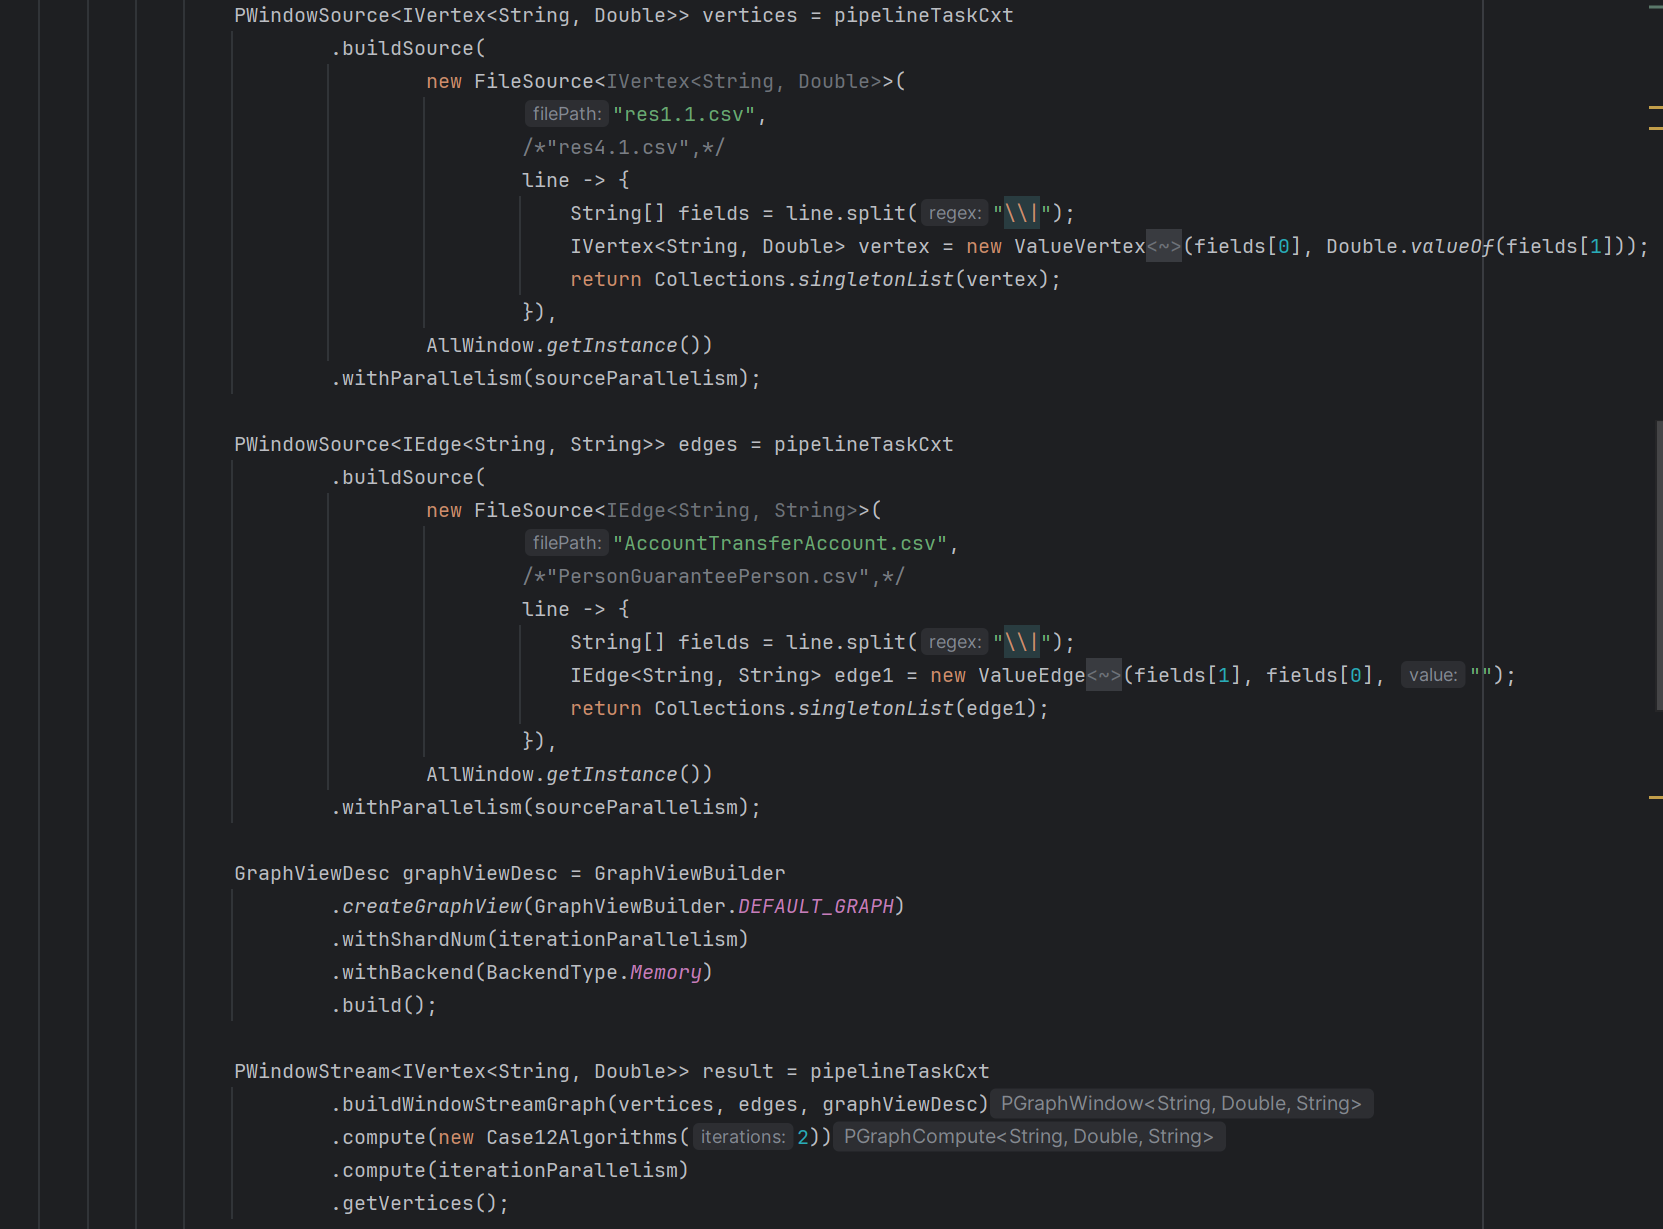
\includegraphics[width=0.85\textwidth,scale=0.7]{./figures/pro4/4.png}
  \end{center}
\end{figure}

接着我们进行两轮迭代,与第一次处理类似,将点的value值根据边往前传递。
需要注意的是,为防止未经过transfer的点在最后一轮也被计算进去,在传递前先让所有点
都向自己的接收器发送0.0(接收器没有值的点不会进入第二轮迭代),并在第二轮迭代中
进行更新value值,这样就只有通过边传递值的account的value值不为0。核心代码如下:
\begin{figure}[H]
  \begin{center}
    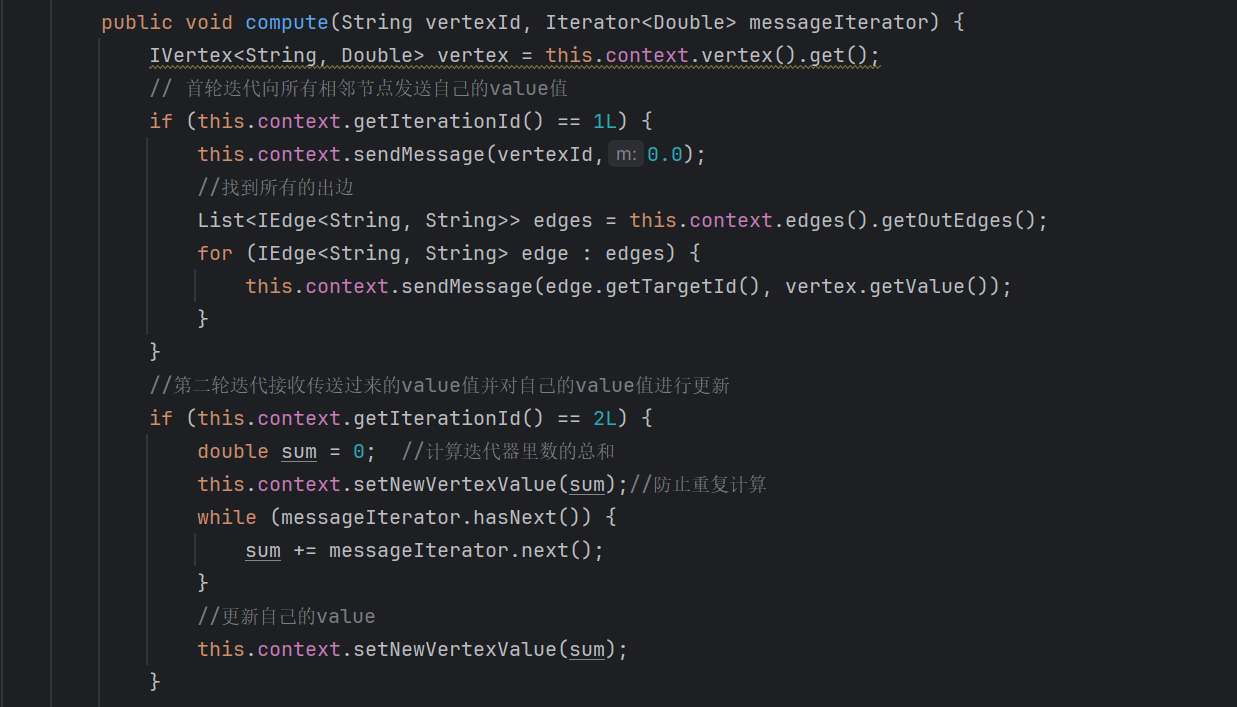
\includegraphics[width=0.85\textwidth,scale=0.7]{./figures/pro4/5.png}
  \end{center}
\end{figure}

第二次中间文件输出格式如下:
\begin{figure}[H]
  \begin{center}
    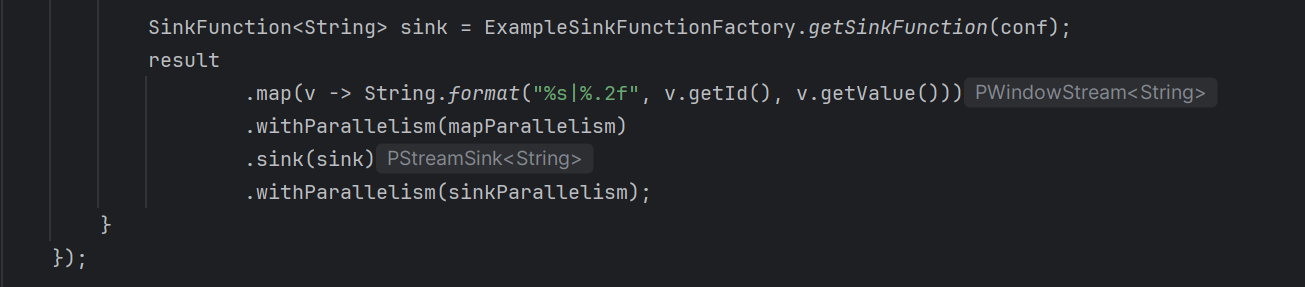
\includegraphics[width=0.85\textwidth,scale=0.7]{./figures/pro4/6.png}
  \end{center}
\end{figure}

接着进入第三步操作,首先我们将中间文件与personownaccount文件和person文件联合起
来构建成图,点的id为account或者person的id,点的value为account的value,person的
value置为0,边的value为空字符串:
\begin{figure}[H]
  \begin{center}
    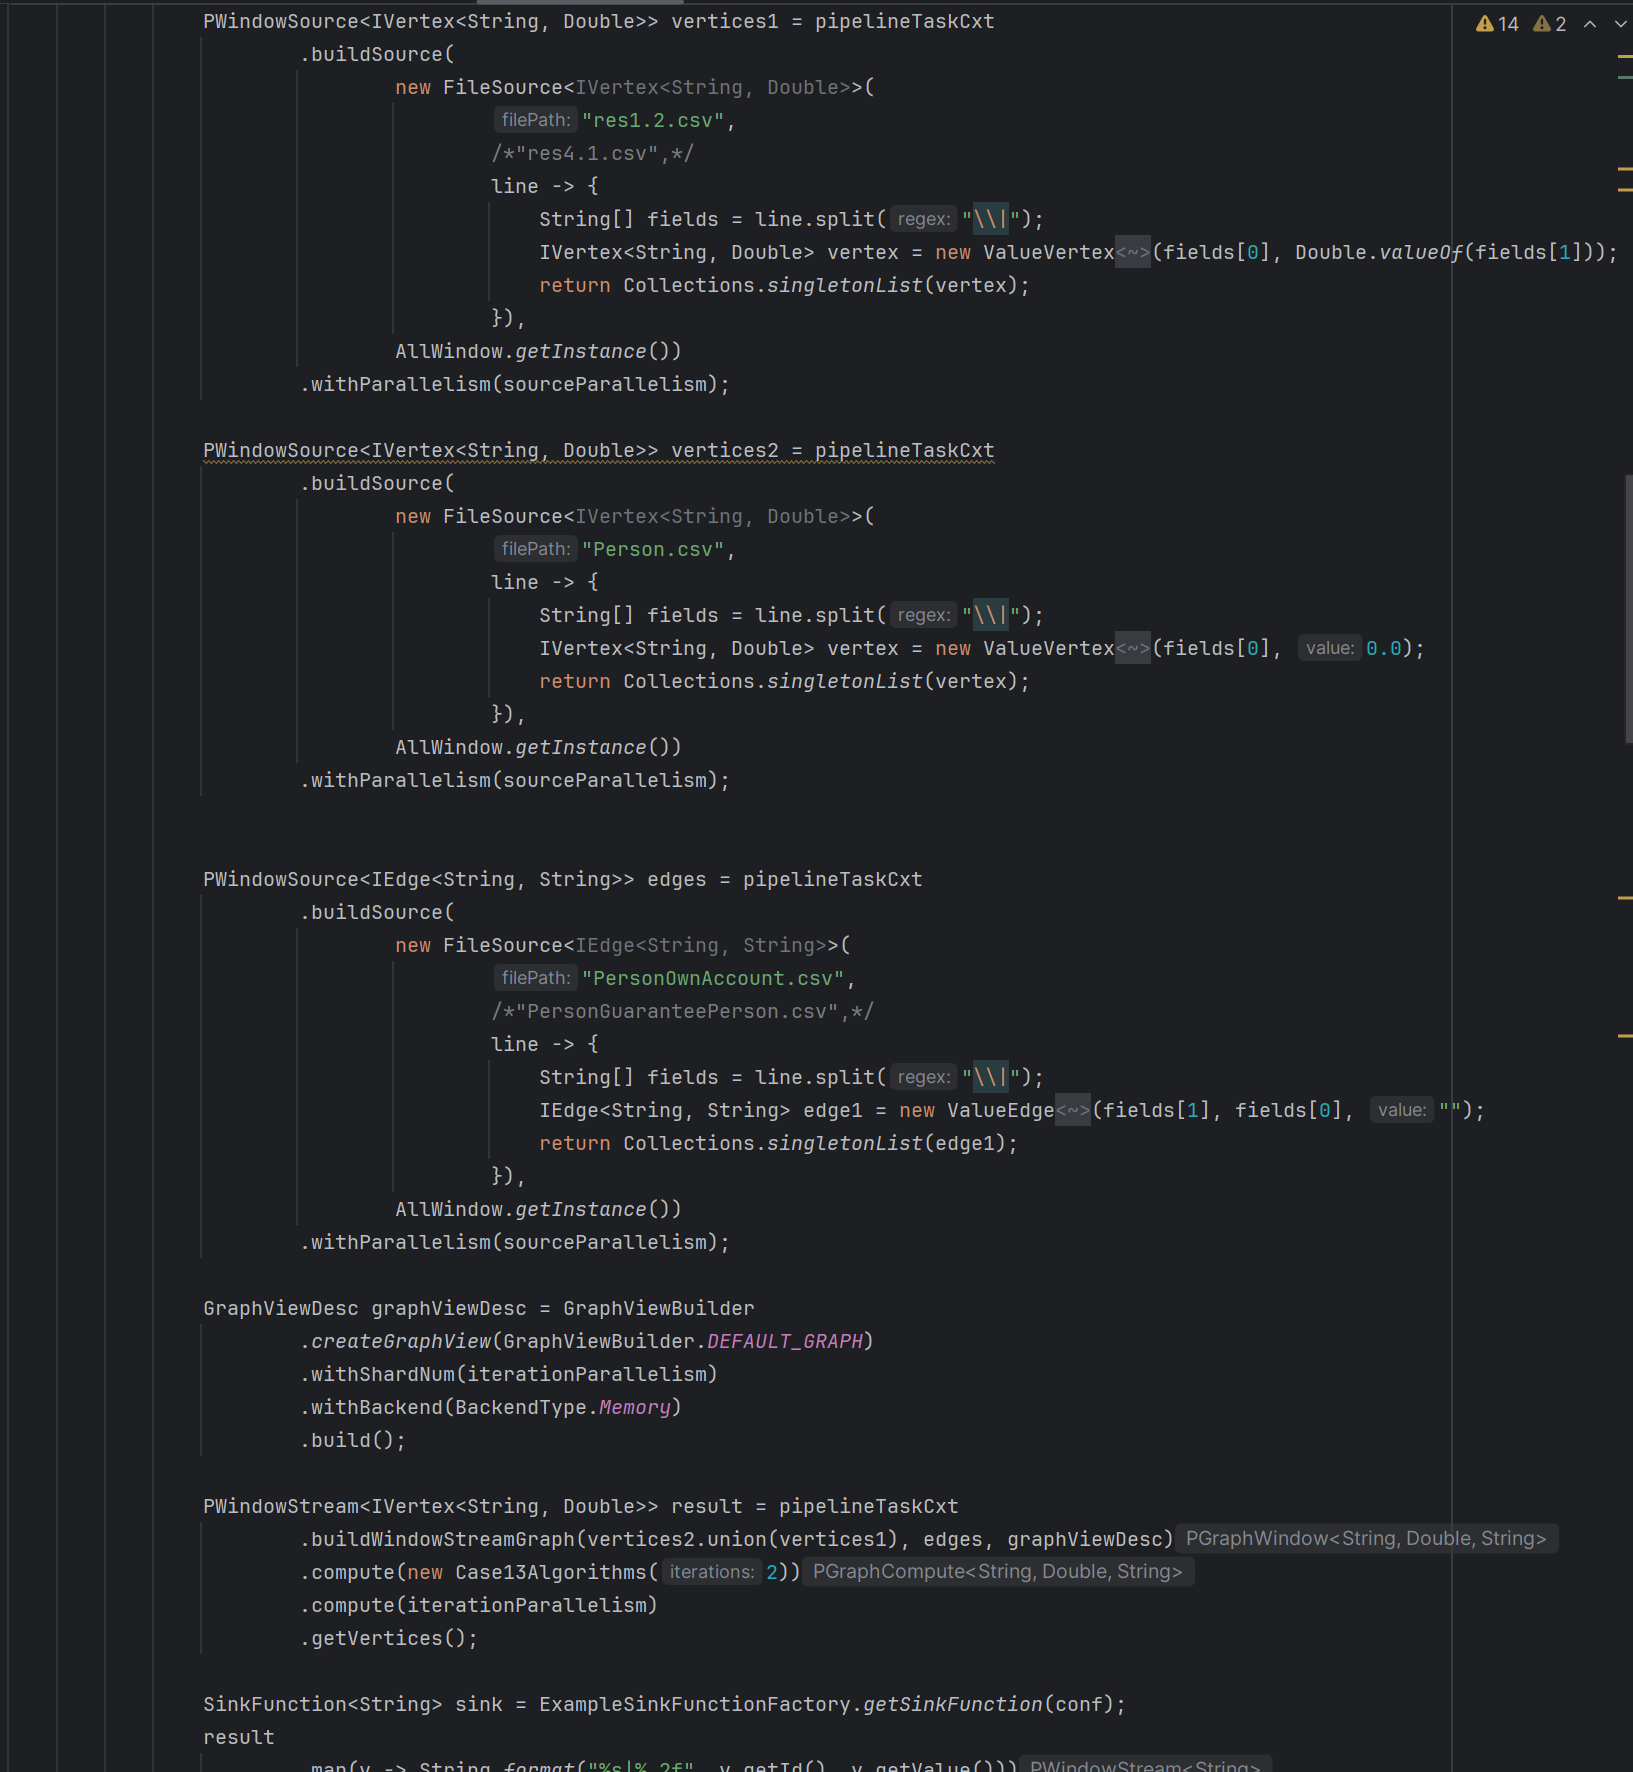
\includegraphics[width=0.85\textwidth,scale=0.7]{./figures/pro4/7.png}
  \end{center}
\end{figure}

接着我们进行两轮迭代,与第二次处理类似,将点的value值根据边往前传递。
不过这次将所有点发送的值为 $ -1 $,用于后续将account点筛选掉。核心代码如下:
\begin{figure}[H]
  \begin{center}
    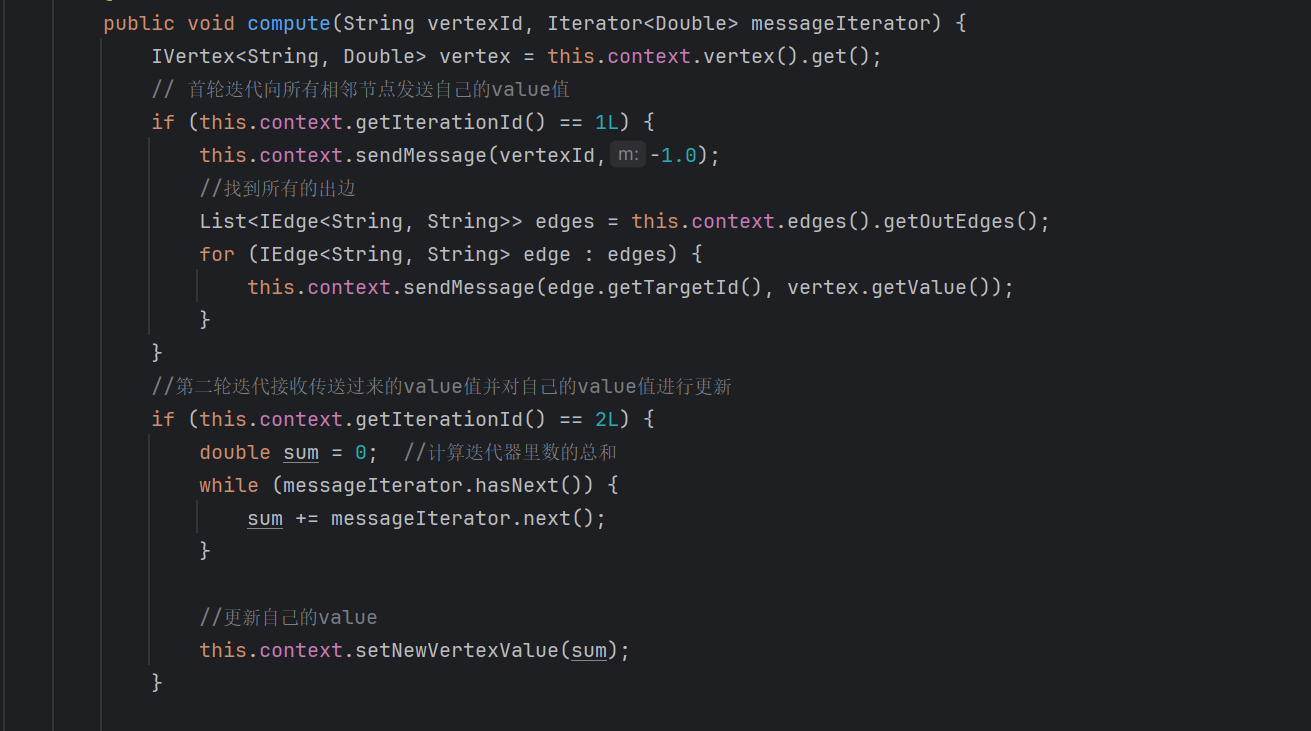
\includegraphics[width=0.85\textwidth,scale=0.7]{./figures/pro4/8.png}
  \end{center}
\end{figure}

最后将结果后保存到文件中
\begin{figure}[H]
  \begin{center}
    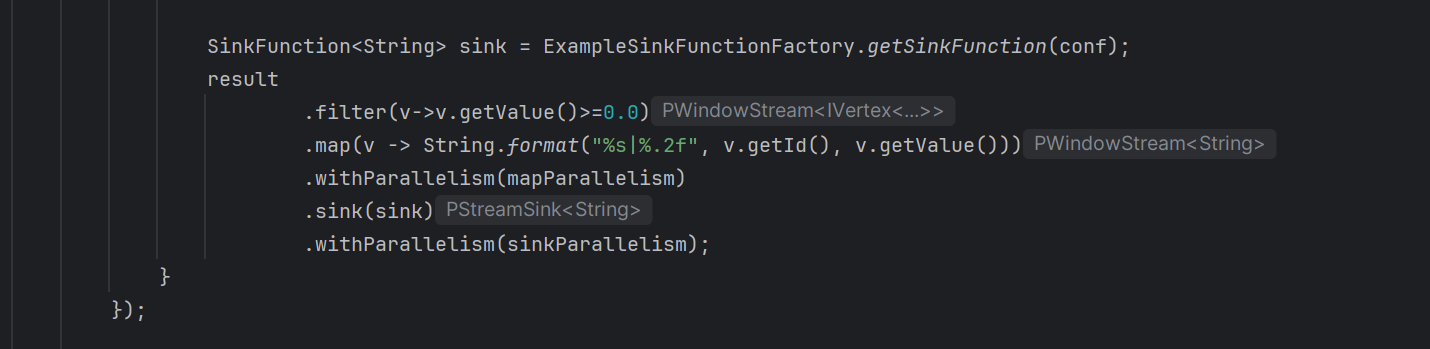
\includegraphics[width=0.85\textwidth,scale=0.7]{./figures/pro4/9.png}
  \end{center}
\end{figure}

但是,提交结果以失败告终了。
我们尝试自己创建文件将自己能想到的所有情况进行测试,结果均正确。但是依然过不了测试,宣告本题以失败告终。但是在尝试过程中也收获了许多知识点。



%3 XXX
%(具体研发的纸质基础、技术、算法、模块…)
%4 XXX
%(具体研发的纸质基础、技术、算法、模块…)
%( 该部分是课程实践的主要内容,可以根据子任务划分情况,书写多个章节,更多的章
%节等自行添加…)

% 实践总结
% (描述所完成的任务结果情况,以及可能的特色与应用意义、价值等,以及通过课程学习
% 和实践,一些其他方面的收获或成果等….)
\section{实践总结}
在这次 CCF-BDCI 竞赛中,我们参与了基于 TuGraph Analytics 的高性能图模式匹配算法设计的大数据项目。这个项目是基于蚂蚁集团开源的分布式实时图计算引擎 TuGraph Analytics。在现代大数据应用场景中,图模型被引入作为一种高效地处理大量 Join 操作的数据模型。我们的主要任务是在测试数据集上利用分布式图计算引擎提供的迭代计算框架来实现大规模图数据上的图模式匹配算法,并尽可能提升这些算法的整体性能。我们共同提交了对这四个问题的解决方案,尽管有些问题的解决方案最终未能够通过官方数据集的评测,但仍然从中学习到了许多宝贵的经验。

\subsection{交易闭环搜索问题}
我们的目标是找出图中所有形成闭环的账户。这个问题的核心算法是寻找图中三角形$ K^3 $的个数。
我们首先通过构建点和边来创建图视图,然后实施了一种消息传递算法。
每个点 $ A $ 会向所有相邻点发送消息,并且当这个消息在图中传递时,消息的内容会根据边的连接方式发生变化,计算消息三次传递后仍然返回原点的闭环数量,顺利通过了官方数据集评测。

这种方法让我们深入理解了图计算的核心思想和消息传递机制。我们学会了如何有效地在图结构中传递信息,并且学会使用迭代器来处理图结构中的信息传递机制,对我们解决以下几道题目起到了巨大的帮助。

\subsection{资金快进快出问题}
这个问题的目标是找出所有账户的资金流入流出比。我们主要需要对图中每个点的入边和出边的处理。
我们首先构建了点和边来形成图视图,然后使用迭代计算来找出每个点的资金流入流出比。
顺利通过了这道题目的评测。

在这个过程中,我们学会了如何处理和分析涉及大量交易的图数据。特别是,我们了解到了如何在图模型中实现复杂的计算,这对于理解现实世界中的金融交易网络非常有帮助。

\subsection{担保金额汇总问题}
\textbf{初始算法}:我们的目标是汇总所有符合特定条件的人的贷款金额。我们的初始算法包括两个主要步骤:首先连接 Person.csv 和 Loan.csv 文件,生成一个包含个人ID和此人申请的贷款总额的新表。接着,我们使用这个新表和 PersonGuaranteePerson 表来分析满足条件的人的信息。我们使用图迭代和消息传递算法来实现这一过程,提交后未能通过官方评测但我们考虑到数据集中可能存在环形情况而我们算法无法解决这个问题因此我们改进了算法。

\textbf{改进后的算法}:在反思我们的初始方法后,我们改进了第二步的计算方法,通过封装点为对象,并将传递的数据类型改为字符串类型,以便更好地控制信息流并去重。我们通过四轮迭代的方法来累加所有符合条件的人的贷款金额。尽管我们的改进在自己选择的测试集中表现良好,但最终仍未能通过官方的评测。

尽管我们没有解决这个问题,但我们从中学到了如何处理图中的环形结构,以及如何优化图计算算法以提高性能和准确性。
我们还学到了在面对复杂问题时如何进行迭代改进和创新的重要性。

\subsection{个人贷款统计问题}
\textbf{图构建和数据准备}:我们首先创建了一个基于图的数据结构,这涉及将多个数据源整合为图中的点和边。为了保证数据的准确对应和防止ID冲突,我们采用了特定的策略来区分不同类型的点。

\textbf{迭代计算过程}:我们设计的算法核心是通过多轮迭代计算来传递和聚合数据。在每一轮迭代中,点会根据其连接的边,传递或接收特定的数据值。这个过程涉及了对每个点的值进行更新和累加,以此来实现从一级点到下一级点的数据传递。

\textbf{结果生成与优化}:最终,我们通过过滤和汇总操作生成所需的结果。虽然我们的算法在自我测试中表现良好,可以通过我们设置的数据集,但在官方评测中未能成功,或许在处理边界情况和特殊场景时,我们仍有未考虑到的情况,但由于时间以及能力有限,我们没有再对算法进行优化改进。

% 参考文献
% (给出相应参考文献,注意书写好格式,参考毕业设计论文要求)
\begin{thebibliography}{99}
\bibitem{ref1} \href{https://tugraph-analytics.readthedocs.io/en/latest/}{GeaFlow 官网}
\bibitem{ref2} \href{https://github.com/TuGraph-family/tugraph-analytics}{GeaFlow 代码仓库}
\bibitem{ref3} \href{https://arxiv.org/pdf/2306.15975.pdf}{LDBC FinBench⽂档}
\bibitem{ref4} TuGraphAnalytics. \href{https://zhuanlan.zhihu.com/p/650101776}{TuGraph任务能⼒增强:通过API定制流图计算逻辑}
\bibitem{ref5} Reinhard Diestel. Graph Theory, Fifth Edition.
\end{thebibliography}


\end{document}
